%Basic Page Formatting%
\documentclass[12pt,twoside]{report}
\usepackage[letterpaper,margin=1in,bindingoffset=0.25in]{geometry}
\usepackage[utf8]{inputenc}
\usepackage[english]{babel}
\usepackage[babel]{csquotes}
\usepackage{titling}
\usepackage[protrusion=true,expansion=true]{microtype}
\usepackage{setspace}
\onehalfspacing
\usepackage{appendix}
%Chapter Styling%
\usepackage{titlesec}
\titleformat{\chapter}
{\normalfont\Large\bfseries}{\thechapter.}{18pt}{\Large}

%Fancy Page Styling%
\usepackage{fancyhdr}
\pagestyle{fancy}
\fancyhead{}
\fancyhead[RO,LE]{Thesis Title}
\fancyhead[RE,LO]{Chapter \thechapter}
\fancyhead[C]{}
\fancyfoot{}
\fancyfoot[LE,RO]{}
\fancyfoot[C]{\thepage}
\setlength{\headheight}{15pt}

%Reference Management%
\usepackage[
backend=biber,
style=chem-acs,
articletitle
]{biblatex}
\addbibresource{references.bib}

%Image Formatting%
\usepackage{graphicx}%Enchanced graphics support%
\usepackage{float}%Float options$
\graphicspath{{./figures/}}

%Math Formatting%
\usepackage{amsmath}%AMS Math%
\usepackage{amsthm}%Theorem Formatting%
\usepackage{amssymb}%AMS Symbols%
\usepackage{array}%Allows for more complex matrices
\usepackage{siunitx}%Formats SI units%
\usepackage{booktabs}%Typsets tables%
\newcommand{\specialcell}[2][c]{\begin{tabular}[#1]{@{}l@{}}#2\end{tabular}}
\newcommand{\specialcellbold}[2][c]{%
	\bfseries
	\begin{tabular}[#1]{@{}l@{}}#2\end{tabular}%
}
\usepackage{chemformula}

%Lorem Ipsum%
\usepackage{lipsum}

\begin{document}

%Title Page%
\begin{titlepage}
	\begin{center}
		\vspace*{1.5 cm}
		\textbf{\{Working Title\}}


		\vspace{1.5 cm}

		by\\ Benjamin Bui
		\vspace{1.5 cm}

		Professor Peacock-Lopez, Advisor
		\vspace{1.5 cm}

		A thesis submitted in partial fulfillment\\
		of the requirements for the\\
		Degree of Bachelor of Arts with Honors\\
		in Chemistry
		\vspace{1.5 cm}

		Williams College\\
		Williamstown, Massachusetts
		\vspace{1.5 cm}

		\today
	\end{center}
\end{titlepage}


\setcounter{page}{1}
\thispagestyle{plain}
\begin{center}
	\vspace*{\fill}
	\textbf{Acknowledgements}\\
	I would like to express my gratitude to my advisor, Professor Enrique Peacock-L\'opez for supporting me throughout my thesis. It was always helpful to have someone I could bounce ideas off of and to explain to me obtuse math I would find in the literature. You really let me develop and understand the material needed independently but were always there when I needed help. You were the first professor I did research with in the summer of my freshman year and it was a pleasure to work on my thesis with you in my senior year.
	
	I would also like to thank my suite and the people of the Jesup community for providing me with both the emotional and technical support throughout my thesis. You provided the breaks after long hours of work and I look forward to staying close to all of you long after I graduate

	Thank you to the faculty and students Chemistry Department of Williams College. I have worked with, under, or even helped tutored many of you and I hope that you all continue to do fantastic work inside or outside of chemistry. I understand that my thesis appears unorthodox for the department but I thank you all for being understanding and willing to let me work on this. 

	I of course must mention my family who were instrumental in raising me and helping reach the point I am now. Thank you to my mother and father, to my brother and sister: Helen and Bryant, and to the rest of my extended family to whom I love dearly.
	\vspace*{\fill}
\end{center}
\pagebreak
\thispagestyle{plain}
\begin{center}
	\vspace*{\fill}
	\textbf{Abstract}\\
\end{center}
	Dynamical systems are present in a variety of fields including the study of economics, physics and chemistry. The study of stochastic dynamical systems was pioneered by Louis Bachelier\autocite{Bachelier1900} who attempted to model Brownian motion to study financial systems although it was later popularized by Einstein and developed into the theory of statistical mechanics. Econonomic and financial models quickly began adapting these theories into their own models with the field of econophysics being developed in order to accomodate these and related ideas. Many notable processes in chemistry and physics are represented as chaotic dynamical systems; however, chaos is still not a commonplace point of discussion in macroeconomic theory. In this paper, I present two previously created business cycle models, a multiplier-accelerator model with a Robertson lag by T\"onu Puu and an inventory cycle model with a Lundberg lag by Metzler and Wegener, before creating a new model that incorporates these elements from these two models. This model explains the inability for firms to accurately determine future outcomes on the potentially chaotic or quasi-periodic behavior of output levels. I find that even given reasonable parameter choice, it is reasonable for the model to be in a chaotic regime, thus allowing business cycles to be driven endogenously as opposed to through external, stochastic shocks.
	\vspace*{\fill}
\pagebreak
\tableofcontents
\chapter{Introduction}
The study of dynamical systems is traditionally thought to have begun with the publication of "New methods of Celestial Mechanics" by Poincar\'e and expanded with the work of Lyapunov into a theory of the stability of dynamical systems. It was not until the 1960s however that the use of chaos and stability theory exploded across disciplines\autocite{Aubin2002}. 

Dynamics are typically an unnecessary tool when studying the paths of chemical reactions. Their value became apparent however, when Belousov and later Zhabotinsky released published their work on an oscillatory reaction, a reaction that would later come to be known as the BZ reaction\autocite{Winfree1984}. Cycles were also known to exist in the biochemical realm with many famous pathways in organisms such as the Krebs cycle and Calvin cycle; however the BZ reaction was developed to create an inorganic analogue to the Krebs cycle\autocite{Field1986}. The development of this cycle allowed for a relatively easily replicable cyclic reaction with with easily measurable indicators of the progress of the reaction. 

The study of dynamical chemical systems has since expanded to a variety of other mechanisms such as self-replicating molecules\autocite{Beutel2007} in addition to studying fractal patterns and dimensionality involved in electrochemical deposits\autocite{Hudson1994} and flame patterns\autocite{Matalon2009}. Despite the fairly wide range of background information required to set up these different models, the underlying mathematical theory used to study these models is identical which has contributed to the wide range of interdisciplinary work performed by theorists in the field.
\section{Background on Dynamical Systems}
Traditional dynamical systems are modelled in continuous time as a system of ordinary differential equations. These systems typically treat time as the singular independent variable and solve for the evolution of one or more variables in terms of time. A classic continuous time dynamical system is the simple pendulum which allows one to model the movement of a pendulum in space in terms of time. This model uses a variety of simplifying assumptions in order to reduce the problem of the pendulum into a single variable function, holding the length of the pendulum and acceleration due to gravity constant.
\begin{equation}
    \frac{d^2}{dt^2}+\frac{g}{L}\sin\theta=0
\end{equation}
Most  attempts  at  modelling  real-world  systems  however  require  the  use  of  multiple dependent variables in order to effectively model.  However, as the amount of variables increases, the complexity of the model increases.  Modelling and $n$-body system acting on each other gravitationally is of obvious interest in astronomy; however, it was quickly found  that  although  a  1  and  2  body  system  were  relatively  simple  to  solve  for,  the introduction of a third body caused significant complications.  The 3-body system is in fact what Poincar\'e studied in order to develop a theory of chaotic deterministic systems\autocite{Poincare1993}.

That is not to say that these systems cannot arrive at ordered solutions.  Although continuous time systems require a minimum of 3 variables in order for chaos to arise, there are typically windows of order in chaotic regimes that allow for stable, oscillatory behavior. The BZ-reaction is still being actively studied and is known to be actually highly complex but is often reduced into 7 primary sub-reactions\autocite{Field1986}. A great deal of the work involved in studying dynamical systems is actually on finding ways to simplify models in order to arrive at more mathematically tractable systems. The BZ-reaction has been simplified to a 3-variable system that still provides the complex periodicity and chaotic behavior characteristic of the model\autocite{Gyorgyi1992}.

Although many processes in the real-world are more intuitively interpreted as operating as a continuous time  function, there are many  occasions where it is possible and  in fact beneficial to think in a discrete-time sense. The prevalence of this type of system varies depending on the exact field of study; however, it is important to note that when computationally modelling continuous time systems, it is impossible for computers to truly operate with continuous variables and thus even these systems are reduced to technically discrete models.

Population dynamics are frequently analyzed as a discrete time system as opposed to continuous time. It is often of more practical use to interpret $t= 0,1,2,3,...$ as the change in population per year or per season as opposed to determining the change in population over infinitesimally small changes in time. In terms of technique, many of the mathematical principles used in analyzing dynamic systems in continuous time apply to discrete time systems; however, it would be a mistake to assume the two were identical. An important distinction between the two is the nature by which chaos can occur. As described previously, a continuous time system requires 3 or more dependent variables in order for chaos to occur. A discrete time system only requires 1 variable in order to display the same type of chaotic behavior.

The systems discussed throughout this paper will be of the discrete variety due to their nature. Laws pertaining to the physical world are scalable to the infinitesimal degree which allows for their use in continuous models. Economic models do not have a basis in physical laws. It is also important to note that, due to the complexity involved in the human behavior that economic models are trying predict, the exact numerical values of the model are typically of minor concern. The general behavior of the model is significantly more valuable in order to determine the effects of an economic assumption.

The logistic map is regarded as the prototypical chaotic discrete time mapping. The logistic function, which the logistic map is based off of, was developed to study population dynamics but actually garnered widespread use in other disciplines such as the study of autocatalytic reactions, computer science, statistics, and economics\autocite{Kavanagh1934}.
\begin{equation}
    \frac{d}{dx}f(x)=f(x)(1-f(x))
\end{equation}
The logistic function has 2 equilibria or points where the derivative of the function is 0. $f(x) = 0$ is an unstable equilibrium but $f(x)=1$ is a stable equilibrium point which means that other points on the function will tend towards this equilibrium overtime.  This can be realized by solving for the derivative of the function at points when $f(x)\in(0,1)$ which is universally positive and $f(x)\in(1,\infty)$ which is negative. Integrating the differential equation gives the general form equation:
\begin{equation}
    f(x)=\frac{e^x}{e^x+C}
\end{equation}
This function gained prominence due to its rapid, exponential growth when $f(x)$ is low and its slow, linear decaying to non-existent growth as population increases.  Used by notable mathematicians operating in the field of population dynamics such as Verhulst, Pearl, and Lotka, the model continues to be widely used today and is often the basis upon which other modifications are applied\autocite{Zwanzig1973}.

\begin{equation}
    x_{t=1}=\mu x_t(1-x_t)
\end{equation}
The logistic map is a difference equation model popularized by Robert May as a discrete time analogue to the logistic function\autocite{May1976}. When interpreted in the biological context, $x_t$ refers to the ratio of the population at time $t$ compared to the maximal population, thus the mapping is bounded between 0 and 1. Here we see intuitively the major difference between difference equation and differential equation based systems. Differential equations solve for the derivative of a variable with respect to time in terms of the variable, difference equations solve for the actual state of the variable in the successive state provided we know the state of the variable in the previous time period. Much like how differential equations can be of higher order with the introduction higher order derivatives, a difference equation can also be of higher order by including more time periods in the function for the state of the variable which is valuable in a variety of the models discussed later.

Much like how the equilibrium points were solved for in the differential equation, difference equations also have equilibrium points where $x_{t+1}=x_t$. Interestingly, unlike the logistic function, there does not exist a fixed point at $x_t=1$ as this would result in $x_{t+1}=0$. Solving for the fixed points, we have:
\begin{equation}
    x_{t+1}=x_t=0,\frac{\mu-1}{\mu}
\end{equation}

The stability of a fixed point is again dependent on the derivative of the function; however, there are differences in the details of our analysis. Treating $f(x)=x_{t+1}$, we see the derivative of the logistic map is:
\begin{equation}
    f^\prime(x)=\mu(1-2x)
\end{equation}
For reasons that will become clear later, the stability of a point on the map requires that $|f^\prime(x)|<1$. Solving for when this is true for our two fixed points, we see that $\mu<1$ provides stability for the origin fixed point and $1<\mu<3$ gives stability for the non-zero fixed point. Thus, provided the parameter $\mu$ satisfies either of the conditions set previously, it will converge to one of the fixed points in a relatively small, finite amount of iterations. 

\begin{figure}
    \centering
    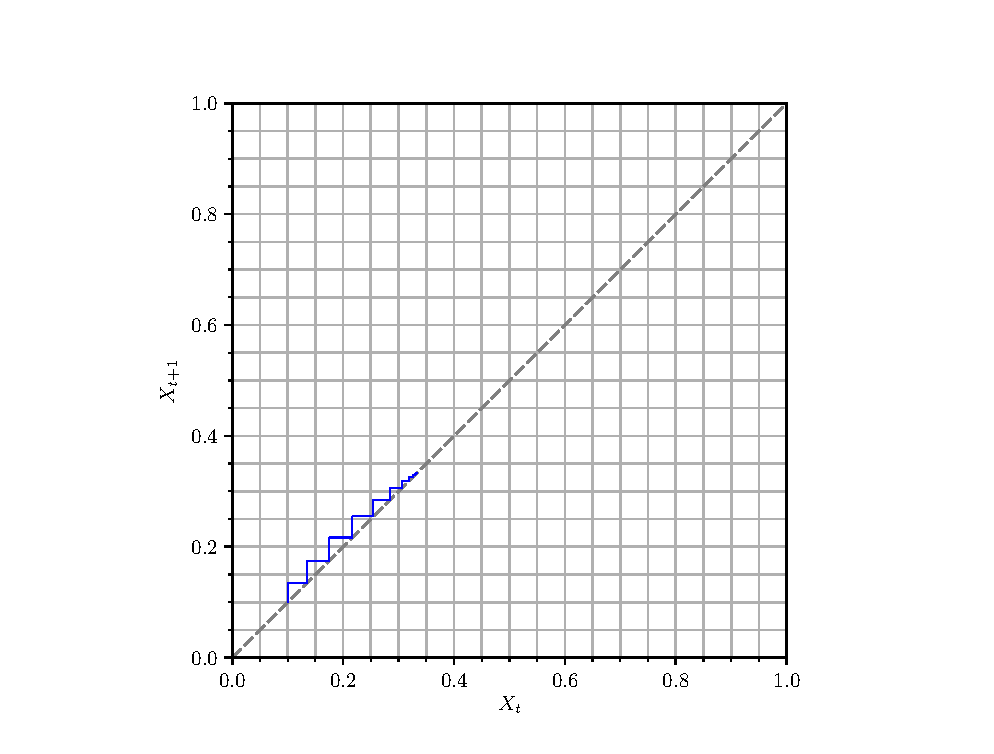
\includegraphics[height=0.4\textheight]{./logistic/fixed_cob.eps}
    \caption{Cobweb plot of the logistic map setting $\mu=1.5$ and $x_0=0.1$. The trajectory asymptotically approaches the equilibrium point of $\frac{1}{3}$.}
    \label{log_fixed_cob}
\end{figure}

This behavior can be visualized using a cobweb diagram. This diagram consists of 3 primary elements: a plot of the mapping, a \SI{45}{\degree} line, and a plot of the variable's trajectory. An example of a cobweb diagram can be seen in Figure \ref{log_fixed_cob}. This diagram shows the trajectory of $x$ starting at a value of 0.1 when there is a stable, non-trivial fixed point.

The \SI{45}{\degree} line is defined as the line where $x_t=x_{t+1}$ which is useful for determining the result of successive iterations. Beginning from the point $x_0$, we can then determine what point $x_1$ wll be via the mapping. We can then look horizontally to the \SI{45}{\degree} line until we intersect with it. The $x$-coordinate of this intersection point is equivalent to the result of the mapping of the previous iteration, thus using this new point will allow us to determine the result of the next iteration of the function. This process can be repeated ad infinitum; however, the result will soon prove uninteresting for stable points and orbits as the trajectory will converge and repeat its behavior.

The reason the logistic map is so frequently studied is because of its ability to exhibit complex behavior beyond a stable equilibrium solution. Once $\mu>3$, the mapping enters a cyclic region. Much like how fixed points could be solved for by identifying where $x_{t}=x_{t+1}$, stable oscillatory points can be found by solving for the equilibrium points of higher iterations of the function. A 2-cycle will be such that $x_{t}=x_{t+2}\neq x_{t+1}$ for example and the stability of a such a cycle can be found using the same methodology as described previously. 
\begin{figure}
    \centering
    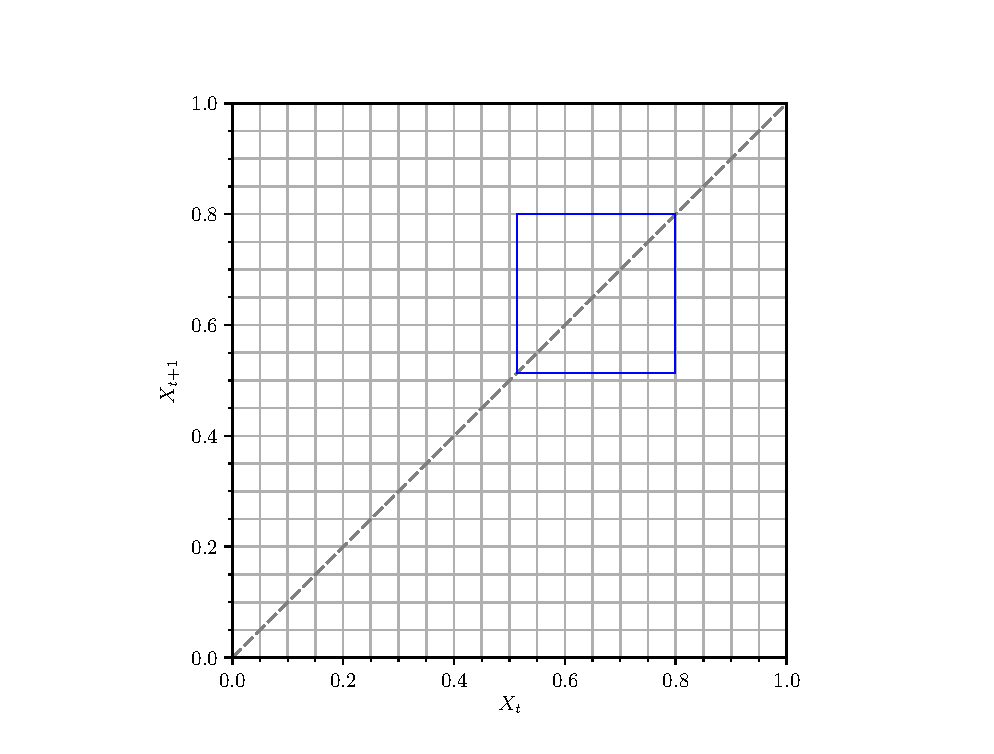
\includegraphics[height=0.4\textheight]{./logistic/2-cyclic_cob.eps}
    \caption{2-period cycle of the logistic map showing only the cyclic behavior.}
    \label{log_cyclic_cob}
\end{figure}
The logistic map also provides a mechanism to more quantitatively describe what it means for a system to be chaotic. The Lyapunov exponent, named after one of major driving forces in the development of stability analysis, is used to measure the effect of small perturbations in initial conditions on the trajectory of the variable\autocite{Puu2003}. Conceptually, the logistic map and the systems discussed in this paper are deterministic. However, chaotic systems have highly divergent trajectories with even small changes in their initial conditions; thus knowing approximately what the initial conditions are does not provide approximate information on the trajectory of the variable. 
\begin{figure}
    \centering
    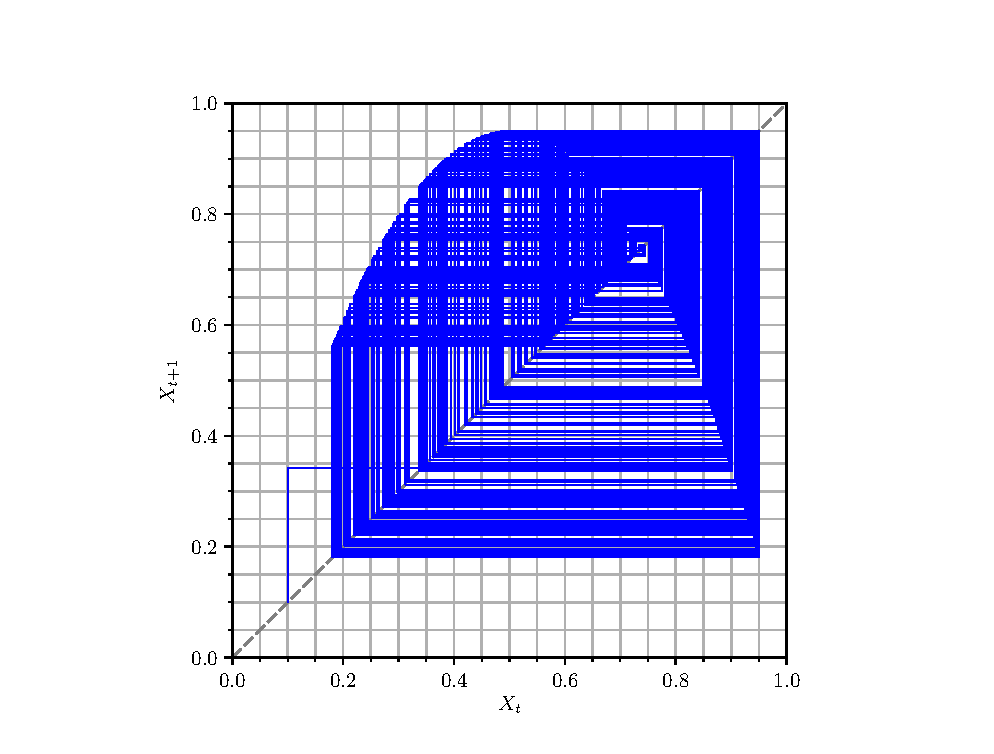
\includegraphics[height=0.4\textheight]{./logistic/chaos_cob.eps}
    \caption{Chaotic behavior in the logistic map.}
    \label{log_chaos_cob}
\end{figure}

In order to quantify this, we begin by taking the absolute value of the derivative of the function as this allows us to effectively magnify the effect of an infinitesimal change in the initial conditions. We then take the natural logarithm of this derivative in order to measure the exponential rate of separation of trajectories. Finally, we take the average separation over an arbitrarily high number of iterations $n$ as exponential separation is not necessitated over all phase space. This gives us a the equation:
\begin{equation}
    \lambda_n(x_0)=\frac{1}{n}\sum^{t=n}_{t=1}\ln\lvert f^\prime(x_{t-1})\rvert
\end{equation}
where $\lambda_n(x_0)$ is the lyapunov exponent for a given initial point when allowed to run for $n$ iterations. The true value of the lyapunov exponent is the limit of the infinite series as $n\rightarrow\infty$ divided by $n$; however, the complexity of these maps often makes it practically impossible to analytically solve for the limit. By choosing arbitrarily high values of $n$ though, it is possible to achieve better approximations at the expense of computational time. It is also important to note that, although the lyapunov exponent is a function of the initial condition, as long as the initial state is not in some stable fixed point or cycle, the trajectories will follow that of the chaotic attractor, thus the value of the lyapunov exponent should be mostly consistent regardless of the choice of initial conditions.
\begin{figure}
    \centering
    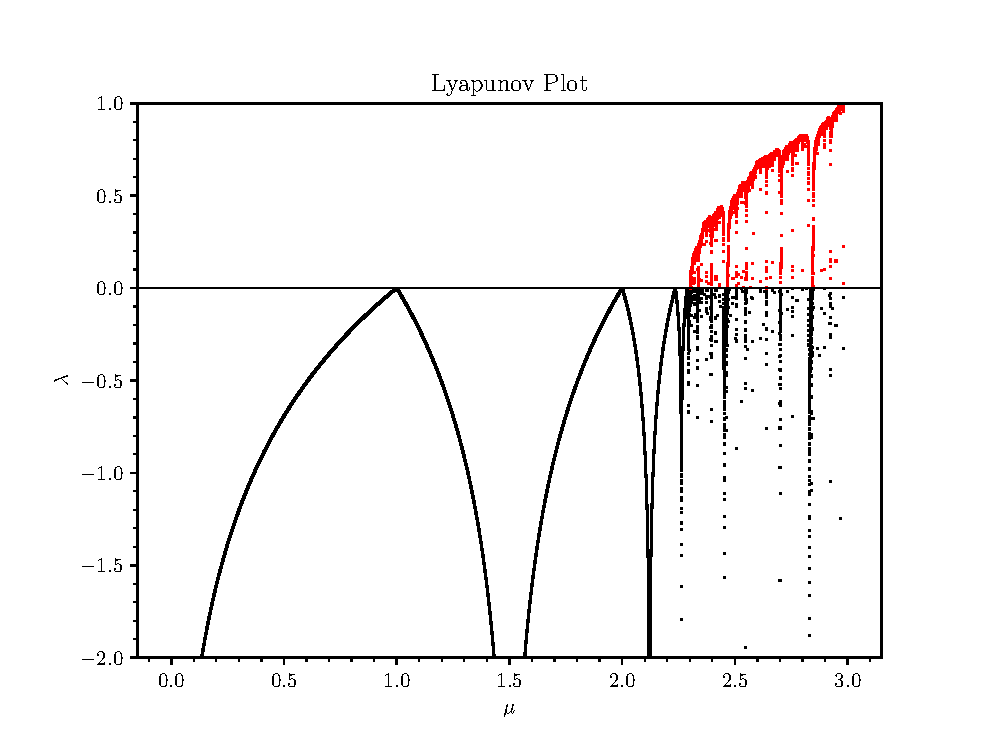
\includegraphics[height=0.4\textheight]{./logistic/lyapunov.eps}
    \caption{Lyapunov exponent plotted against $\mu$ for the logistic map. Initial value of 0.1 is used. Red denotes regions where $\lambda\geq0$, black denotes regions where $\lambda<0$.}
    \label{log_lyapunov}
\end{figure}

Another way visually see the behavior is with a bifurcation diagram. This diagram shows the long run behavior of the variable for a given variable. Figure \ref{log_bifurcation} qualitatively shows the behavior described previously. For parameter values between 0 and 1, we see the origin fixed point is stable. For parameter values between 1 and 3, their is still a single fixed point that is monotonically increasing; however, we can also clearly see the beginning of the 2-period cycle once the parameter exceeds 3. It is difficult however, to determine when predictable higher-order cyclic behavior ends and chaotic behavior begins via qualitative observation of the bifurcation diagram. The benefit of the bifurcation diagram is that it allows us to see both where the bifurcation points are and what behavior the bifurcation points signify. Bifurcation points are 
where where infinitesimally small quantitative changes in the parameter induce significant qualitative or topological change in the behavior of the mapping such as the transition from a stable fixed point to a 2-period cycle. 
\begin{figure}
    \centering
    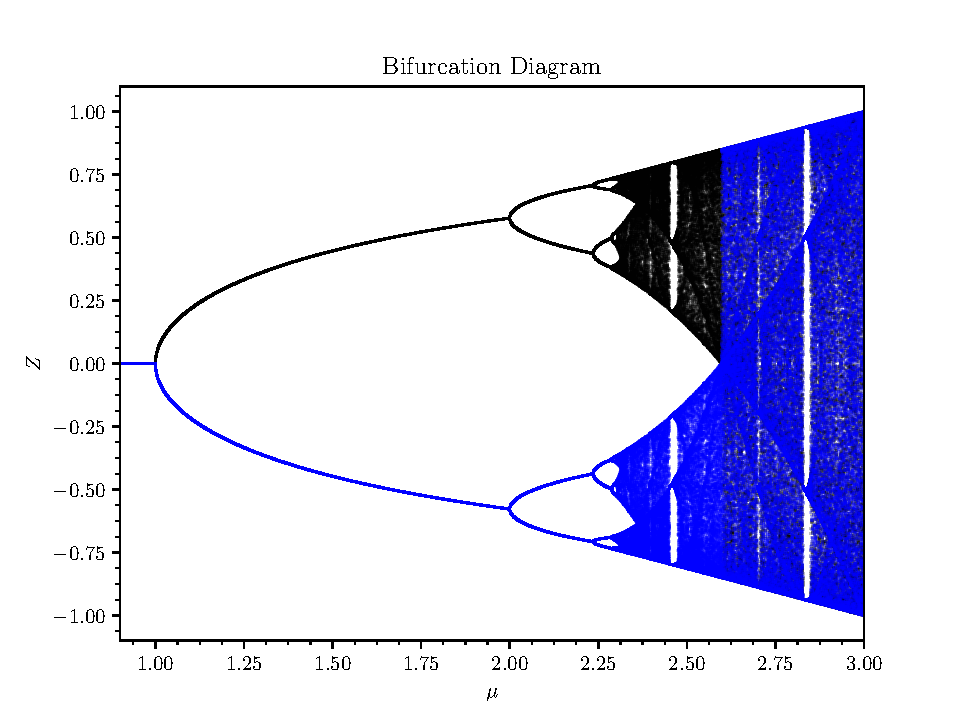
\includegraphics[height=0.4\textheight]{./logistic/bifurcation.eps}
    \caption{Bifurcation diagram plotting $x$ against $\mu$ for the logistic map.}
    \label{log_bifurcation}
\end{figure}

Research on the logistic map and other iterated maps has shown the existence of what is called Feigenbaum's constant. This constant can be found by observing the behavior of the periodic cycles of the map. The interval of stability decreases and the ratio of subsequence intervals actually approaches a limit $\delta\approx4.6692$\autocite{Puu2003}. All other topologically similar maps with a single local maximum share this Feigenbaum constant. Once the mapping exceeds this constant, chaos occurs which allows for another method to determine precisely where chaotic behavior occurs. 

It is also beneficial to point out that another mechanism exists for cyclic behavior to exist. The previously described method involved taking a mapping and solving for the stability of its double iteration. This allows for $2n$-period stability cycles to exists. However, there does exist odd-ordered cycles such as the $3$ cycle; however, it occurs as a window of order in the region of chaos. These windows can be seen in Figure \ref{log_lyapunov} where the Lyapunov exponent dips into the negative region past the chaotic bifurcation point. These bifurcation points are known as tangent bifurcations.
\begin{figure}
    \centering
    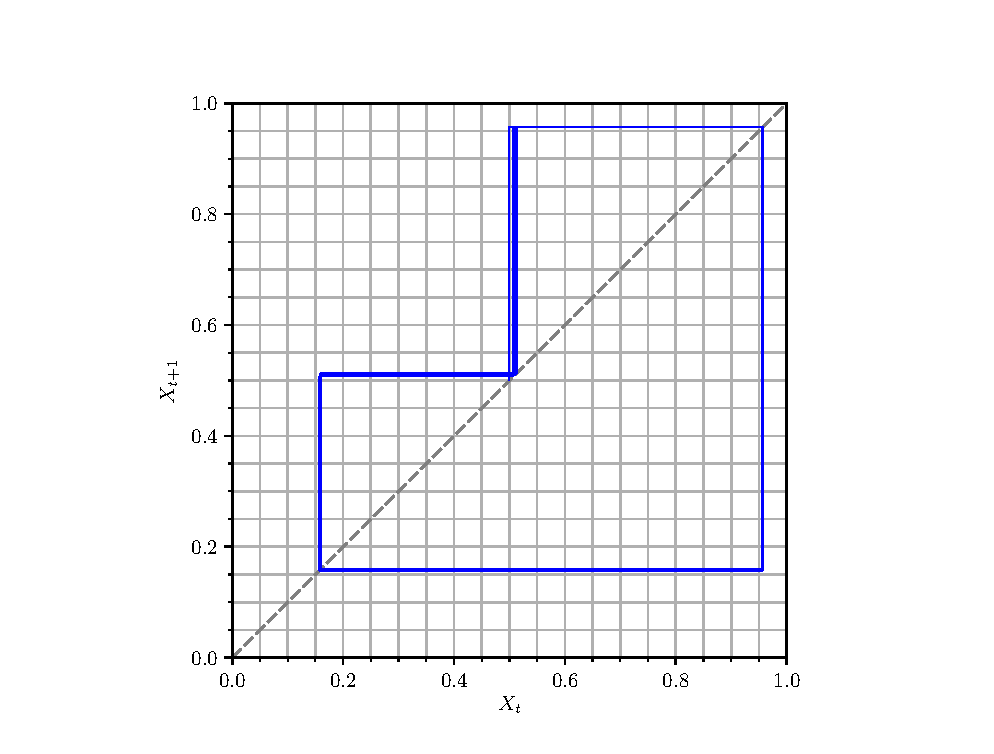
\includegraphics[height=0.4\textheight]{./logistic/3-cyclic_cob.eps}
    \caption{3-period cycle of the logistic map showing only the cyclic behavior.}
    \label{log_3-cyclic_cob}
\end{figure}
This also allows us to use Sharkovsky's Theorem, which states that any continuous mapping with a 3-period cycle must also have every $n$-period cycle for every $n\in\mathbb{Z}$.\autocite{Puu2003} A variety of other mathematical techniques exist to study the dynamics of difference equation mappings but these will be covered more specifically when used for the specific case. 




\chapter{Heterogenous Inventory Cycles by Westerhoff et al.}
\section{Background}
Although nobel prize winning Paul Samuelson was widely credited with providing a mathematical basis to Keynesian economics and popularizing the neoclassical synthesis, he was far from the ony economist involved in the movement\autocite{Skousen1997,Samuelson1939}

Another notable Keynesian was Lloyd Metzler who developed a type of multiplier-accelerator business cycle. This type of model allows for cyclic behavior to occur endogenously, that is to say the model allows for persistent behavior outside of the steady state. This idea runs contrary to the idea that economic booms and recessions are reactions to exogenous shocks which is common in the new classical models. Also known as freshwater economics, these models assume that agents are perfectly rational and are capable of learning from past experiences. This viewpoint came into prominence in the late 1970s with a model by Lucas and Sargent\autocite{Lucas1979} which sought to move past these seemingly outdated Keynesian principles. In the modern day however, Keynesianism has regained popularity with a new neoclassical synthesis that resulted in a new school of thought, New Keynesianism, that seeks to provide stronger micro-foundations to macroeconomic models than was previously encountered in neo-Keynesianism. 

Many models developed in the neo-Keynesian era of economics still remain in use but have either been expanded or used to study specific relationships. Wegener, Wegener, and Zaklan expand upon Metzler's inventory cycle model by introducing heterogenous expectations into firm behavior\autocite{Wegener2009}. 

Unlike the well known multiplier-accelerator model developed by Samuelson and Hicks, the dynamics of this model are driven by shifts in the heterogenous mix of behaviors in the firms. This model reduces the decision of firms to one of two behaviors, a regressive type and an extrapolative type. The extrapolative behavior occurs when a firm predicts that future income will deviate from the long-run average. The regressive behavior occurs when firms predict that future income will return to the long-run average. It is this heterogeneity as well as the ability for firms to switch their behavior type that is the defining feature of this model. 

\section{Model Set-Up}
In this business cycle model, the economy is closed and income is determined completely by the quantity of goods produced by firms. Goods are completely homogenized but can be produced for 3 purposes: stock $S$, consumption $U$, and investment $I$. This lets us define income as:
\begin{equation}
    Y_t=I_t+S_t+U_t
\end{equation}
Investment is held to be exogenously determined and constant, thus:
\begin{equation}
    I_t=\bar I
\end{equation}
Consumption adapts to income according to the marginal propensity to consume, $b$. As this model follows closely to the framework developed by Metzler\autocite{Metzler1941}, consumption adapts directly to the current income level as follows:
\begin{equation}
    C_t=bY_t
\end{equation}
Producers have a desired level of inventory based on the expected level of consumption goods. Thus setting, $k>0$:
\begin{equation}
    \hat Q_t=kU_t
\end{equation}  
where $Q$ is the level of inventory. In order to achieve this desired level of inventory, firms produce $S$ amount of output such that:
\begin{equation}
    S_t=\hat Q_t-Q_{t-1}
\end{equation}
However, the expected level of consumption does not necessarily match the produced level of goods. The realized level of inventory change can thus be determined as:
\begin{equation}
    Q_t=\hat Q_t-(C_t-U_t)
\end{equation}

The quantity of goods produced for consumption is determined by firms expectations for desired consumption. The extrapolative expectation rule is used by firms that believe consumption levels will continue shifting away from the long-run average quantity. This behavior is interpreted mathematically as:
\begin{equation}
    U^E_t=C_{t-1}+c(C_{t-1}-\bar C)
\end{equation}
where $c\geq 0$ denotes the speed at which firms expect consumption to deviate from the long-run level. 

The other possible strategy firms can take is to expect consumption to return to the equilibrium level. This is described as the regressive expectation rule and is interpreted mathematically as:
\begin{equation}
    U_t^R=C_{t-1}+f(\bar C-C_{t-1})
\end{equation}
where $0\leq f\leq 1$ denotes the expected adjustment speed to the long-run level. 

As this economy only involves two expectation rules, the aggregate expected level of consumption is a simple weighted average:
\begin{equation}
    U_t=w_tU_t^E+(1-w_t)U_t^R
\end{equation}
The weight is defined as a function of consumption level which allows firms to switch their predictive behavior based on the current consumption level. Intuitively, as consumption deviates further from equilibrium, more firms will believe that the boom or slump will end and adjust in accordance. Likewise, when consumption is close to equilibrium, firms will believe it to be more accurate to extrapolate consumption. Weight is determined by the function:
\begin{equation}
    w_t=\frac{1}{1+d(\bar C-C_{t-1})^2}
\end{equation}
where $d$ is determined by the popularity of the regressive rule. 

Taking these rules in aggregate, income is a second-order nonlinear iterated mapping. Condensing the model, we arrive at the mapping:
\begin{equation}
    Y_t=U_t+kU_t-(1+k)U_{t-1}+C_{t-1}+\bar I
\end{equation}
This gives a single fixed point of:
\begin{equation}
    \bar Y=\frac{1}{1-b}\bar I
\end{equation}

It is apparent that, as $\bar Y$ is constant, the theoretical set-up of the model is only valid if their is no long-term growth. This is because the predictive mechanism used by firms is reliant on the difference between the lag in consumption and the steady-state level of consumption. If consumption were to consistently grow, then this difference would also grow over time, eliminating any effective purpose in providing heterogenous expectations as firms would practically unanimously switch to the extrapolative mechanism. 


\begin{figure}
    \centering
    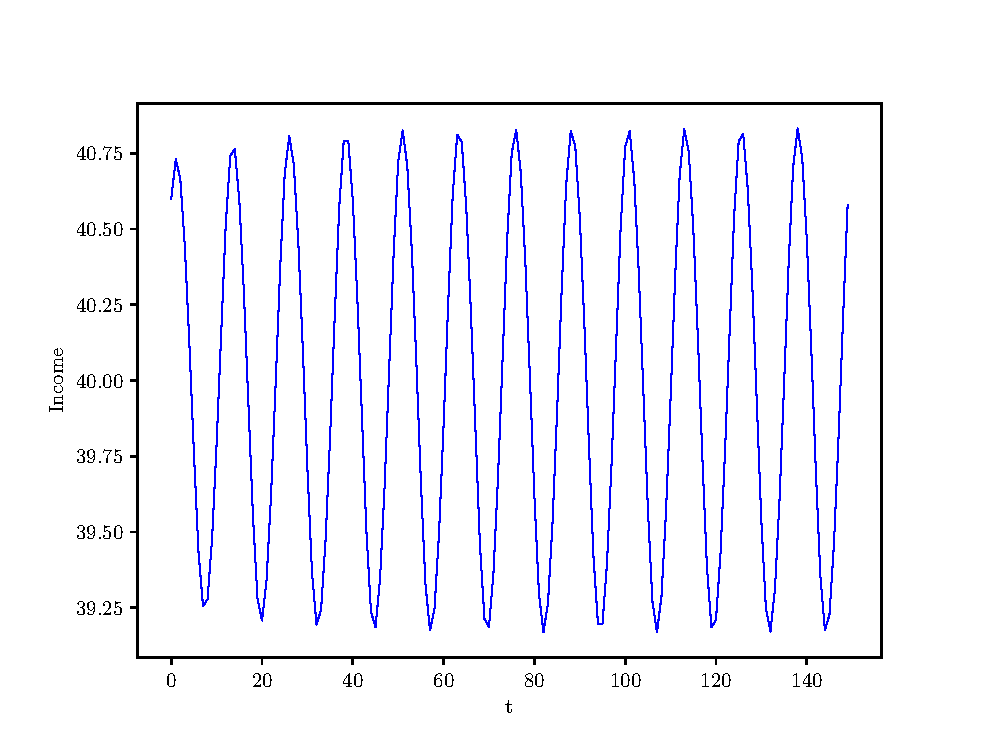
\includegraphics[height=0.4\textheight]{./metzlerian_basic/timeseries_income.eps}
    \caption{Timeseries plot of inventory cycle as described by Wegener et al.\autocite{Wegener2009} Simulation is determined given $Y_0=40.6$, $U_0=30.3$, and $\bar I=10$. The parameters of the model are: $b=0.75,c=0.3,d=1.0,f=0.1,k=0.1$. Income does not feature long-run growth but rather oscillates around the steady state level of income.}
    \label{metzler_basic_timeseries}
\end{figure}

\section{Analysis of Income Dynamics}
In the example trajectory given above, income clearly followed bounded, cyclic behavior. As seen with the analysis of the logistic map however, there are other types of long-term behavior possible. Given the restrictions on parameters, the steady-state level of income is stable if:
\begin{equation}
    k<\frac{1-b-bc}{b(1+c)}
\end{equation}
The proof for this can be seen in the appendix of Wegener et al.\autocite{Wegener2009} The stability of the steady state is only dependent on $b$, $k$, and $c$, thus the behavior of the regressive expectation rule and the ratio of firms behaving with each expectation rule do not affect the stability of this fixed point. This can be seen graphically using bifurcation diagrams of the parameters.

\begin{figure}
    \centering
    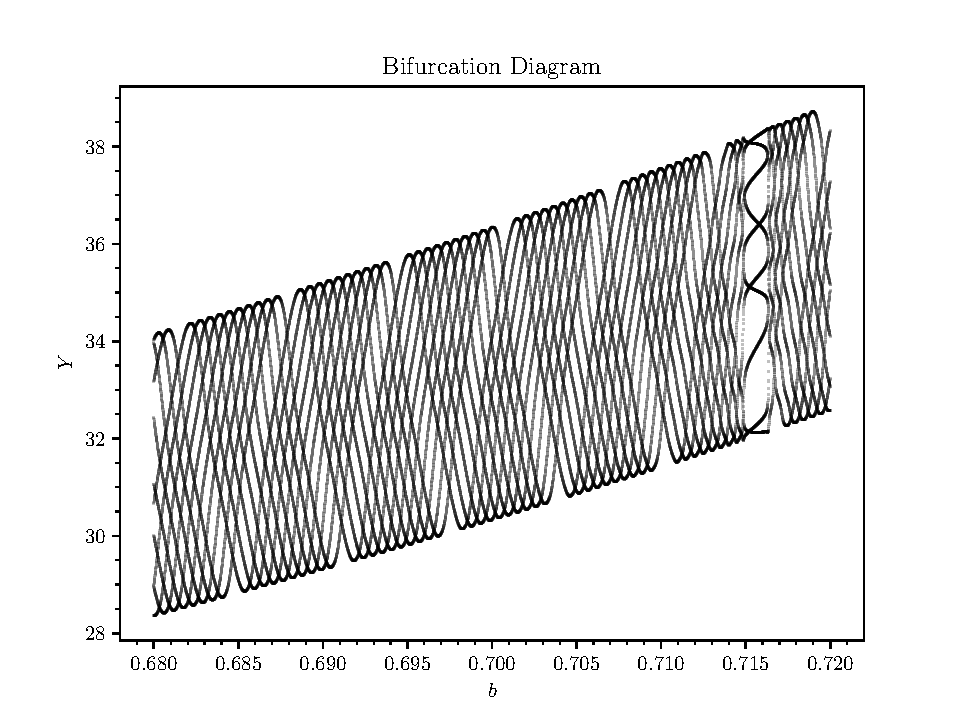
\includegraphics[height=0.4\textheight]{./metzlerian_basic/bbifurcation.eps}
    \caption{Bifurcations diagram varying the parameter $b$ over the range [0.2, 0.85]holding all other parameters and initial conditions as described in Figure \ref{metzler_basic_timeseries}. The simulation was allowed to run for 1000 iterations and the last 50 points are captured in the diagram.}
    \label{metzler_basic_bbifurcation}
\end{figure} 

\begin{figure}
    \centering
    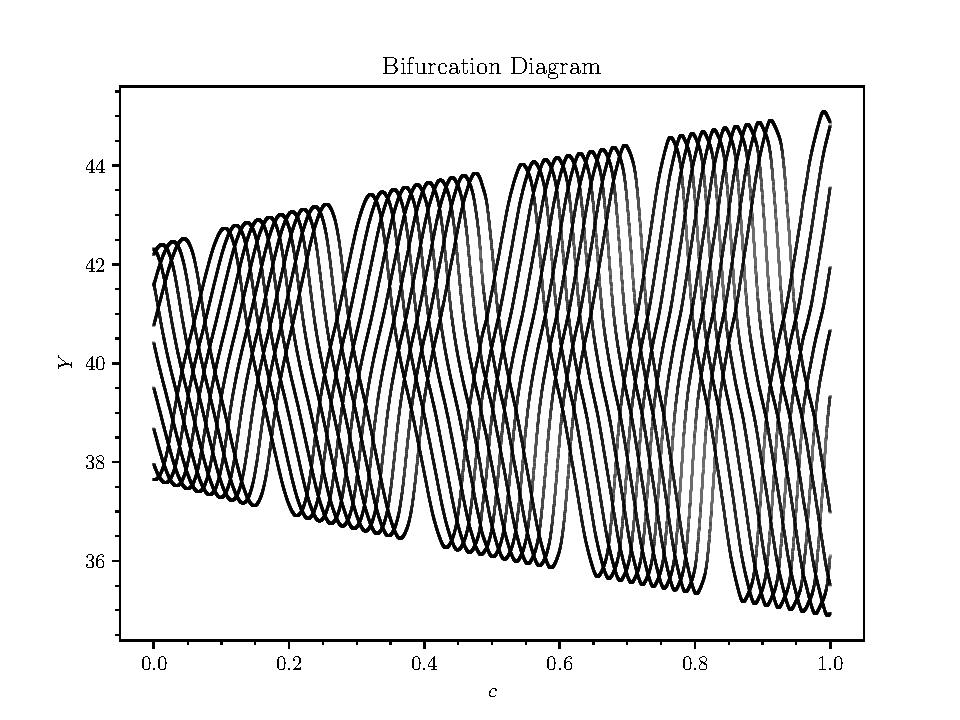
\includegraphics[height=0.4\textheight]{./metzlerian_basic/cbifurcation.eps}
    \caption{Bifurcations diagram varying the parameter $c$ over the range [0.1, 0.9] holding all other parameters and initial conditions as described in Figure \ref{metzler_basic_timeseries}. The simulation was allowed to run for 1000 iterations and the last 50 points are captured in the diagram.}
    \label{metzler_basic_cbifurcation}
\end{figure} 

\begin{figure}
    \centering
    \includegraphics[height=0.4\textheight]{./metzlerian_basic/kbifurcation.eps}
    \caption{Bifurcations diagram varying the parameter $k$ over the range [0.1, 0.4] holding all other parameters and initial conditions as described in Figure \ref{metzler_basic_timeseries}. The simulation was allowed to run for 1000 iterations and the last 50 points are captured in the diagram.}
    \label{metzler_basic_kbifurcation}
\end{figure} 

There is a Neimark-Sacker bifurcation where $b\approx0.65$ which marks a transition point from a stable fixed point to a bounded cycle. However, as $b$ approaches 1, the bifurcation diagram does not graphically feature cycles of well defined order. Varying $c$ and $k$ alters the behavior of the cycles as seen in Figure \ref{metzler_basic_cbifurcation} and \ref{metzler_basic_kbifurcation}. Altering $d$ or $f$ affects the magnitude of the inventory cycles but does not have any effect on the presence of the cycles.

\begin{figure}
    \centering
    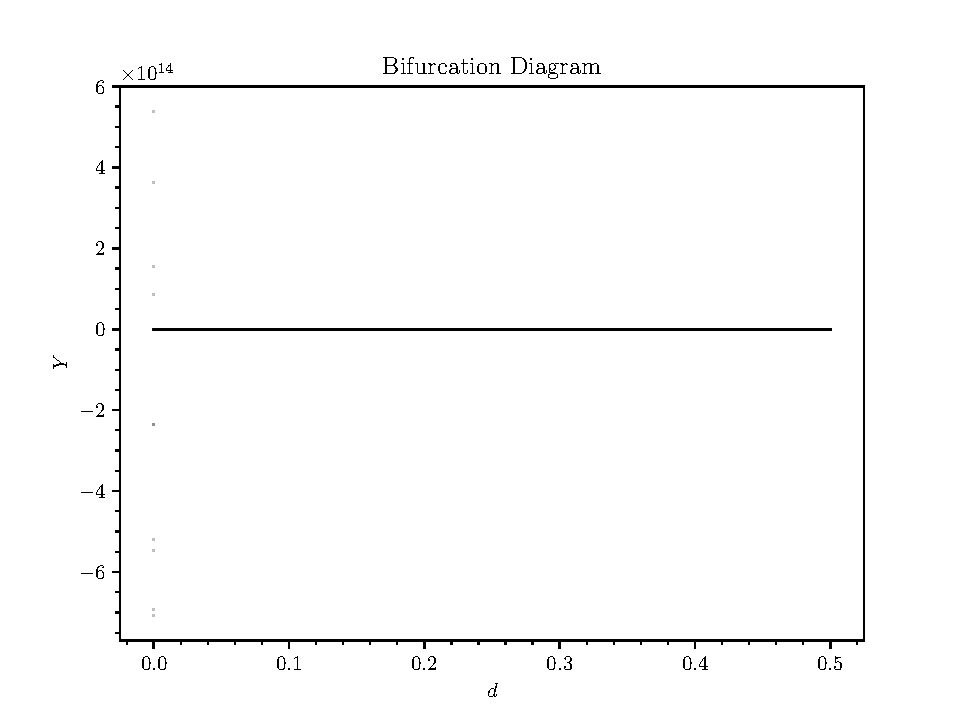
\includegraphics[height=0.4\textheight]{./metzlerian_basic/dbifurcation.eps}
    \caption{Bifurcations diagram varying the parameter $d$ over the range [0.01, 2.0] holding all other parameters and initial conditions as described in Figure \ref{metzler_basic_timeseries}. The simulation was allowed to run for 1000 iterations and the last 50 points are captured in the diagram.}
    \label{metzler_basic_dbifurcation}
\end{figure} 

\begin{figure}
    \centering
    
\includegraphics[height=0.4\textheight]{./metzlerian_basic/fbifurcation.eps}
    \caption{Bifurcations diagram varying the parameter $f$ over the range [0.1, 0.5] holding all other parameters and initial conditions as described in Figure \ref{metzler_basic_timeseries}. The simulation was allowed to run for 1000 iterations and the last 50 points are captured in the diagram.}
    \label{metzler_basic_fbifurcation}
\end{figure}

The bifurcation diagrams varying the $c,\ k,\ d,$ and $f$ parameters appear to display clear cyclic behavior. However, this is actually a product of the graphical display of the bifurcation diagram. The diagram is constructed by iterating the mapping over 1000 time periods and displaying the results of the last 50 time-periods. This results in the appearance of 50-cycles over the span of the bifurcation diagram; however, reducing or increasing the amount of iterations to display likewise changes the apparent periodicity of the cycle.


\chapter{Inventory Cycles with Endogenous Investment\\ and Adaptive Expectations}
\section{Model Set-Up}
Metzler's and Westerhoff's model show that it is possible for endogenous business cycles to be induced through inventory cycles and the failure of firms to accurately predict future consumption. These models were designed to focus on the effects of firm expectations with Westerhoff's contribution consisting of introducing a heterogenous expectation rule that allows firms to switch behavior based on the state of the economy. Both of these models however simplify other aspects of the economy that feature more complex behavior in other business cycle models.

The inventory cycle model features 3 main factors of production: predicted consumption, investment, and inventory. Metzler and Westerhoff holds investment as an exogenously determined constant; however, this is both unrealistic and does not allow for long term endogenous growth. To incorporate a mechanism for endogenously adjusting investment, we take inspiration from the multiplier-accelerator model presented in Chapter \ref{ch:multiplier-accelerator}. 

The problem with the cubic investment function used in that model is that it leads to unbounded behavior in the extremes, much like the linear function. Puu resolves this by ensuring that income growth is bounded by [-1, 1]; this is not the case for our model however. We instead want a function that features similar curvature and behavior as the cubic function but flattens when income change is of significant magnitude. This can be accomplished with the following function:

\begin{equation}
    I_t = \frac{\frac{Y_{t-1}-Y_{t-2}}{v}}{(\frac{Y_{t-1}-Y_{t-2}}{v})^4+q}	
\end{equation}

The behavior of this function qualitatively resembles that of the linear-cubic function described in by Puu when $v,q>0$ and ; however, $\lim_{(Y_{t-1}-Y_{t-2})\to\infty}I_t=0$. This function is at its absolute maximum and minimum when:
\begin{equation*}
    Y_{t-1}-Y_{t-2}=\pm\frac{q^{1/4}v}{3^{1/4}}
\end{equation*}
Thus giving a maximal or minimal investment of:
\begin{equation*}
    I_t=\frac{3^{3/4}}{4q^{3/4}}
\end{equation*}
Intuitively, larger values of $v$ make the function "wider", increasing the range over $Y_{t-1}-Y_{t-2}$ where $I_t$ is not effectively 0. Smaller values of $q$ increases the magnitude of the maximum and minimum of the function, effectively making it taller. $v$ and $q$ cannot be directly attributed to any direct economic phenomena; however, their effect on the function can be interpreted analogously to the properties of the linear-cubic function. The "height" of the function determines the potential magnitude of investment and the "width" determines the rate at which investment, both private and public, react to changes in income.

Metzler describes the existence of two important lags in the study of Keynesian models. The Robertson lag is characterized by making current consumption a function of past income, i.e. consumption behavior lags behind current income. The Lundberg lag however concerns a discrepancy between the income level and the production decision of firms \autocite{Metzler1941} . These lags are named after the two economists D. H. Robertson and Erik Lundberg who developed models that contained only their eponymous lag type. Although both lags are likely to exist in reality, most models only incorporate one lag due to the increased complexity associated with it. Metzler and Westerhoff make use of a Lundberg lag by making income a function of the predicted level of consumption as opposed to actual consumption. T\"{o}nu Puu's model makes use of a Robertson in order to induce endogenous business cycles. Metzler himself does not claim that the Lundberg sequence is any more realistic than the Robertson sequence. Whichever lag has a longer time-period can be treated as of being greater importance but Metzler actually proposes a variety of scenarios that present contradicting conclusions. Suppose that decided their behavior on a quarterly basis but consumers altered their spending behavior with every paycheck, then it is no longer unrealistic to treat the Robertson lag as being of 0 length, i.e. nonexistent. If consumers revise their spending behavior every 6 months to a year, then it would actually be more realistic to include a non-zero Robertson lag while minimizing the Lundberg lag. 

For the purposes of this model, we will include a non-zero Lundberg and Robertson lag. The consumption function is treated exactly as presented in Puu:
\begin{equation}
    C_t=(1-s)Y_{t-1}+sY_{t-2}
\end{equation}
This function incorporates a 1-period Lundberg lag where $s\in[0,1]$ is the marginal propensity to save. This function also contains a 2-period delayed consumption due to the marginal propensity to save, thus all income made in some period $t$ can be though of as being eventually spent in the period $t+1$ and $t+2$. Although intuitive, this explanation is not wholly accurate as the Lundberg lag does not imply saving of income to spend in the next period but rather that spending behavior is influenced only on the information of lagged income level. The choice of $s$ dictates the relative importance of lagged income, a higher marginal propensity to save reduces the impact of income made in the previous time period but increases the effective impact of the income made two time periods ago.  

As the economy is also making use of a Robertson lag, income is not directly a function of consumption as may be seen in other models. Rather, income is viewed from a production standpoint. This is achieved by explicitly defining a predicted level of consumption. Westerhoff and Metzler use an equation similar to the form:

\begin{equation*} 
    U_t=C_{t-1}+\eta(C_{t-1}-C_{t-2})
\end{equation*}
However, this assumes that firms have no way to adapt their coefficient of expectation $\eta$. 

A new predictive mechanism requires that firms have bounded rationality. If firms possessed perfect rationality, then they would be able to perfectly predict consumption levels as consumption is based on lagged income, thus if we wish to maintain our Robertson lag, firms must still have bounded rationality. Another mechanism that firms can use that maintains better "memory" is that of an average. 
\begin{equation}\label{predict}
    U_t = \frac{C_{t-1}+C_{t-2}+C_{t-3}}{3}
\end{equation}
This formulation is an average of the consumption levels of the past 3 time periods. The choice of three time periods is relatively arbitrary and higher order difference equations of the same form can be used; however these higher order formulations can result in a less mathematically tractable model.

Inventory production proceeds as seen in Chapter 2 with firms producing $S_t$ explicitly to maintain Inventory at optimal levels:
\begin{equation}
    S_t = k U_t-Q_{t-1}
\end{equation}
where $Q_t$ is the level of inventory maintained at the end of time $t$ and $k\in[0,1]$. This can be solved for as the sum of the previous inventory level, production intended for inventory, and the difference between production intended for consumption and the actual consumption level:
\begin{equation}
    Q_t=Q_{t-1}+S_t+(U_t-C_t)
\end{equation}

Income level, or output, can thus be written as a sum of production:
\begin{equation}\label{eq:Income}
    Y_t=I_t+S_t+U_t
\end{equation}
However, as income has the capability of sustained growth under this model, it is preferable to analyze the rate of change of income in this model. In Appendix \ref{appendix_growth}, we show that the growth rate of the economy can be interpreted as a single variable, 6th order difference equation on $\dot Y$:
\begin{equation}
    \begin{split}
        \dot Y_{t}& = \frac{\frac{\dot Y_{t-1}}{v}}{\left(\frac{\dot Y_{t-1}}{v}\right)^4+q}-\frac{\frac{\dot Y_{t-2}}{v}}{\left(\frac{\dot Y_{t-2}}{v}\right)^4+q} + \\
        & \frac{k+1}{3}\left[(1-s)(\dot Y_{t-2}-Y_{t-5})+s(\dot Y_{t-3}-Y_{t-6})\right]+(1-s)\dot Y_{t-2}+s\dot Y_{t-3}
    \end{split}
    \end{equation}

\section{Growth Dynamics}
The long run dynamics of the model are highly dependent on the choice of initial conditions. Simulation of the model require a choice of 6 initial values of income change in addition to the parameter choice. If the 6 initial values are equivalent, all future iterations of the mapping are equal to this choice and the model remains in a stable steady state. It both more interesting and realistic then to consider cases where there is variation in initial income growth.
\begin{figure}[ht]
    \centering
    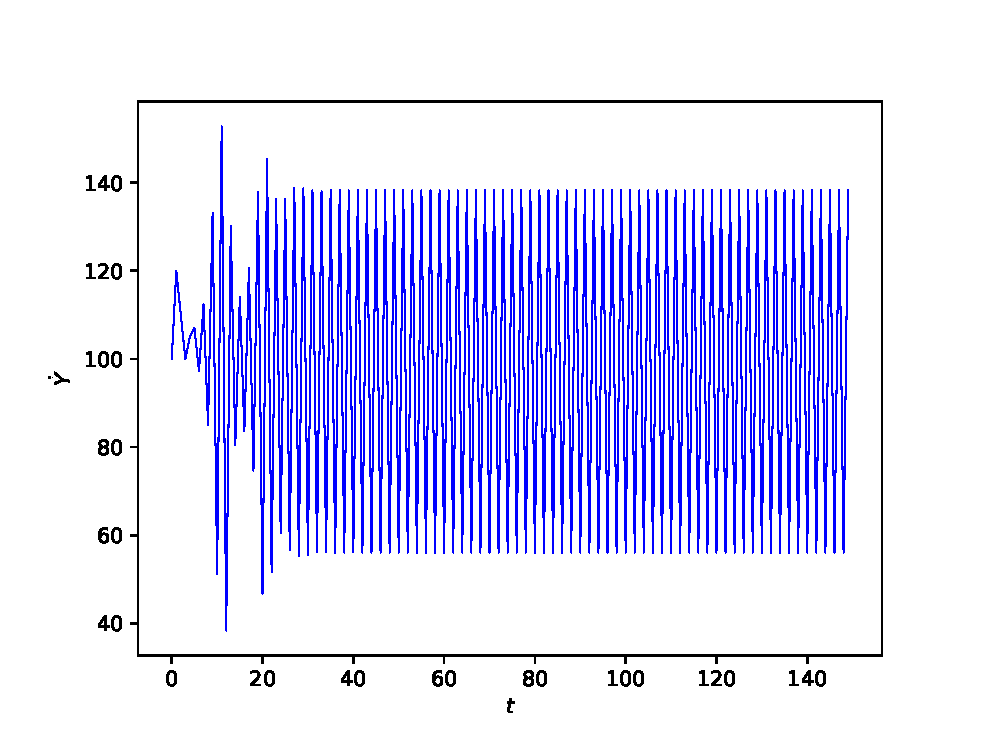
\includegraphics[height=0.4\textheight]{./metzlerian_growth/timeseries1.eps}
    \caption{Timeseries plot of income growth rate over 150 iterations. $s=0.6,\ k=0.3,\ v=500,\ q=0.001$. Initial values of $\dot Y$ are: 100, 120, 110, 100, 105, 107}
    \label{growth_timeseries1}
\end{figure}
Figure \ref{growth_timeseries1} displays a possible trajectory of income growth. Under the parameters listed, the trajectory clearly behaves in a stable, cyclic manner within 40 iterations. 

There do not exist techniques to solve generalized 6th order difference equations; however it is possible to computationally solve for the long run dynamics of the system.
\begin{figure}
    \centering
    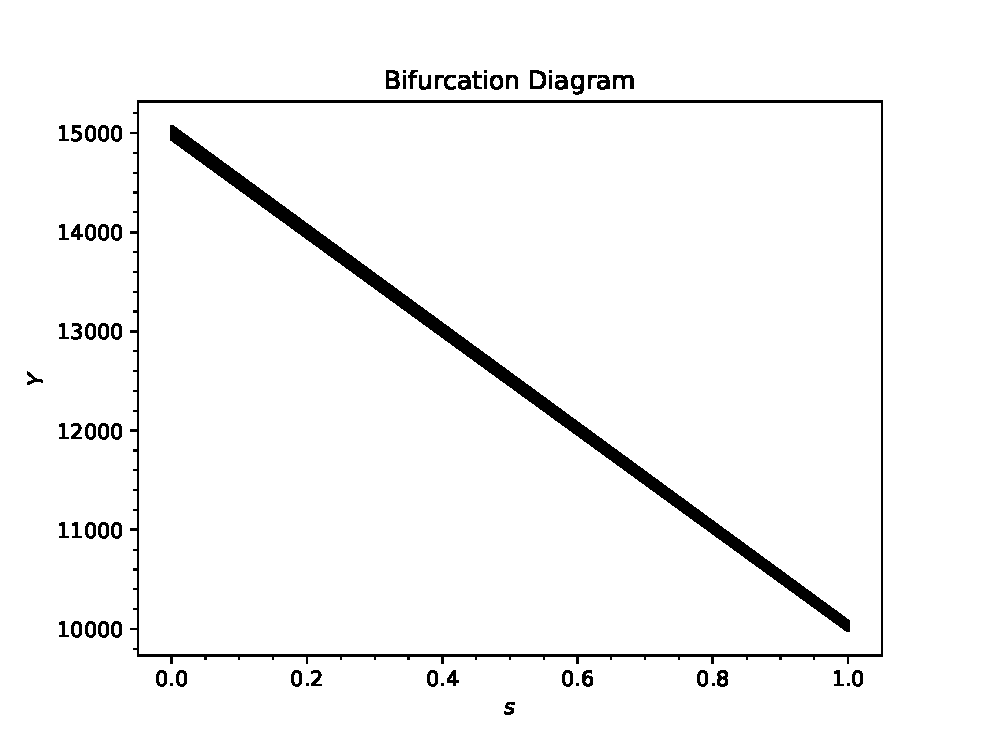
\includegraphics[height=0.4\textheight]{./metzlerian_growth/sbifurcation}
    \caption{Bifurcation diagram varying $s$ between 0.1 and 0.9. Initial conditions and other parameters are held constant as described in Figure \ref{growth_timeseries1}.}
    \label{metzlerian_growth-sbifurcation}
\end{figure}

The bifurcation diagram displayed in Figure \ref{metzlerian_growth-sbifurcation} displays the long-run behavior of the model as $s$ is varied. The methodology of the computational analysis and results are displayed in detail in Section \ref{bifurcation_analyzer} and Section \ref{bifurcation_analysis}, respectively. Long-run values are rounded to their nearest whole number for the purposes of this computational analysis although it is possible to account for higher levels of numerical precision using the analyzer. A bifurcation point exists at $s=0.65$ and $s=0.53$, the mapping is a stable 2 cycle when $s$ is between these two values. This implies the presence of a stable business cycle when the marginal propensity to save is moderately high; however, the behavior appears chaotic when the marginal propensity to save approaches either extreme. 

\begin{figure}
    \centering
    \includegraphics[height=0.4\textheight]{./metzlerian_growth/kbifurcation}
    \caption{Bifurcation diagram varying $k$ between 0.1 and 0.9. Initial conditions and other parameters are held constant as described in Figure \ref{growth_timeseries1}.}
    \label{metzlerian_growth-kbifurcation}
\end{figure}

The bifurcation diagram varying $k$ seen in Figure \ref{metzlerian_growth-kbifurcation} qualitatively appears much simpler than Figure \ref{metzlerian_growth-sbifurcation}. This diagram displays a bifurcation point when $k\approx 0.84837$. The model displays stable 2-cycle behavior until this point although the system continues to display windows of ordered cycles. It thus appears that although increasing the desired proportional level of inventory does increase the long-run level of cyclic growth, it does not affect the topology until $k$ is unrealistically large. 

\begin{figure}
    \centering
    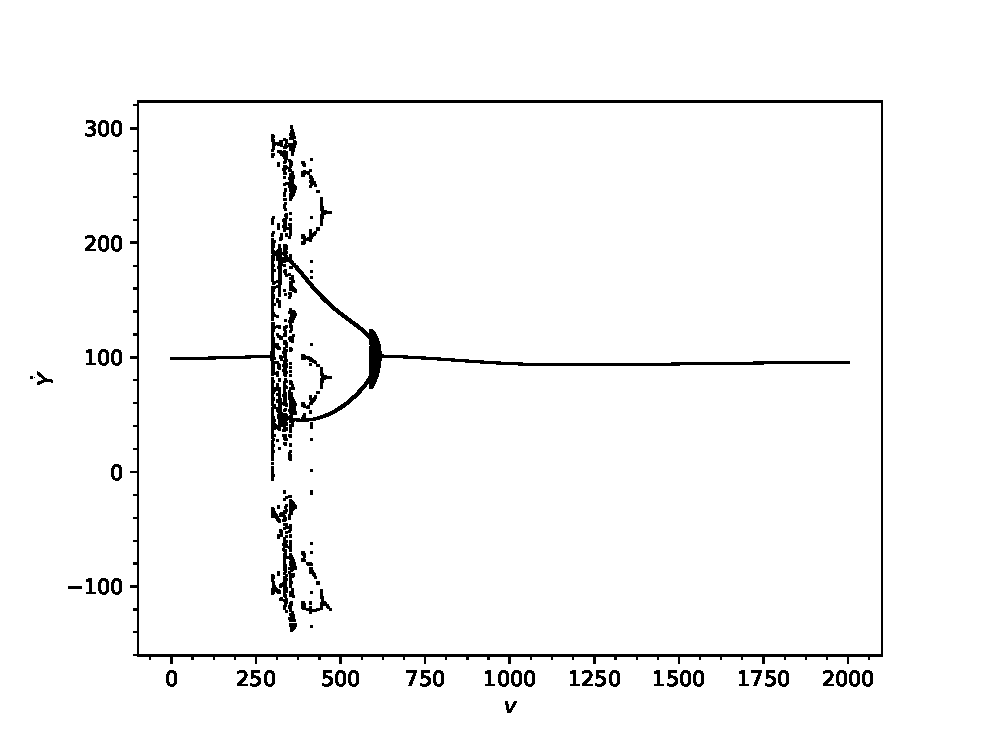
\includegraphics[height=0.4\textheight]{./metzlerian_growth/vbifurcation}
    \caption{Bifurcation diagram varying $v$ between 1 and 2000. Initial conditions and other parameters are held constant as described in Figure \ref{growth_timeseries1}.}
    \label{metzlerian_growth-vbifurcation}
\end{figure}
\begin{figure}
    \centering
    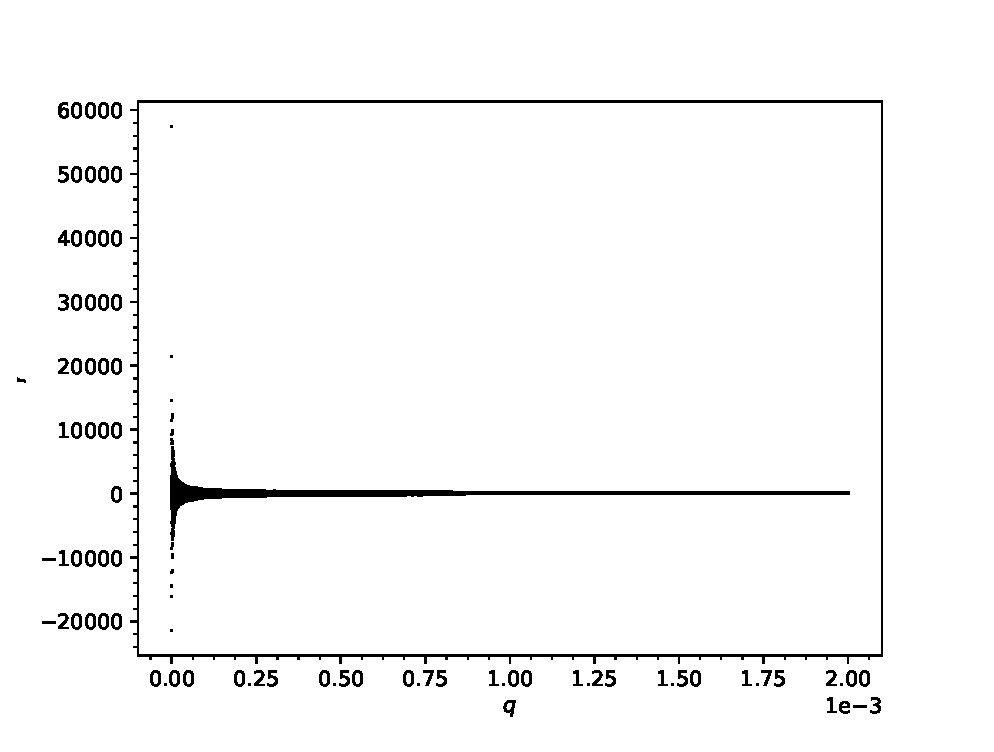
\includegraphics[height=0.4\textheight]{./metzlerian_growth/qbifurcation}
    \caption{Bifurcation diagram varying $q$ between 0 and 0.0001. Initial conditions and other parameters are held constant as described in Figure \ref{growth_timeseries1}.}
    \label{metzlerian_growth-qbifurcation}
\end{figure}

Figure \ref{metzlerian_growth-vbifurcation} exhibits stable, fixed growth when $v\in[1,297.338)\cup(617.104, 2000]$ which is the upper bound of what was computationally determined. The model also displays a stable 2-cycle when $v\in(472.173, 589.757)$. Likewise, Figure \ref{metzlerian_growth-qbifurcation} has a bifurcation point at $q\approx0.0015997$ and $q\approx0.0015976$ which mark transitions from a stable, fixed point to a 2-period cycle to a 3-period cycle (more bifurcation points exist within the diagram and are more easily viewed by narrowing the parameter variation range). As stated previously, $v$ and $q$ individually lack an economic interpretation, but together they approximate the dynamics of a linear-cubic investment curve while incorporating bounded, asymptotic behavior. 

These bifurcation diagrams do not tell the complete story of this model however for any given set of parameters. As stated previously, the choice of constant initial conditions will result in a constant trajectory of income growth. However, it is also trivial to show the existence of other trajectories by creating a timeseries holding the parameters constant but shifting the initial conditions.
\begin{figure}
    \centering
    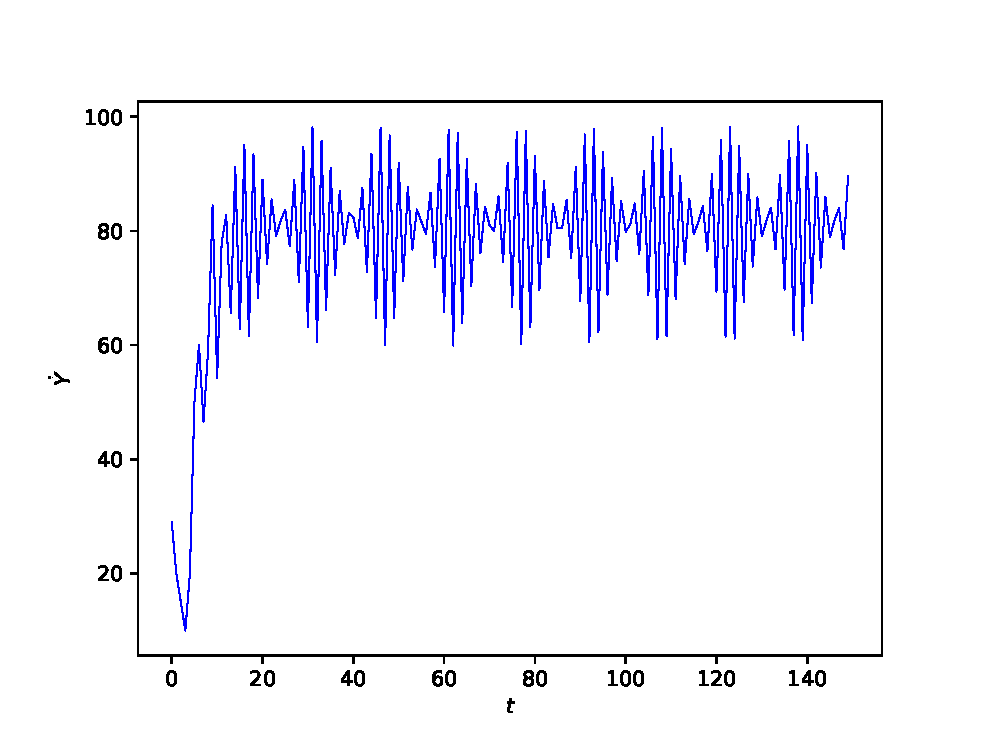
\includegraphics[height=0.4\textheight]{./metzlerian_growth/timeseries3}
    \caption{Timeseries plot of income growth rate over 150 iterations. Parameter choice is identical to that of Figure \ref{growth_timeseries1}. Initial values of $\dot Y$ are: 29, 20 , 15 , 10, 20 ,50,}
    \label{growth_timeseries3}
\end{figure}

The timeseries displayed in Figure \ref{growth_timeseries1} and Figure \ref{growth_timeseries3} share the same parametrization but they clearly display distinct dynamics and are centered around different growth rates. It can be helpful then to think of each initial value as a parameter for the purposes of analysis, thereby allowing us to create bifurcation diagrams in order to identify the effects in the long-run behavior of the model with varying initial conditions. 

\begin{figure}
    \centering
    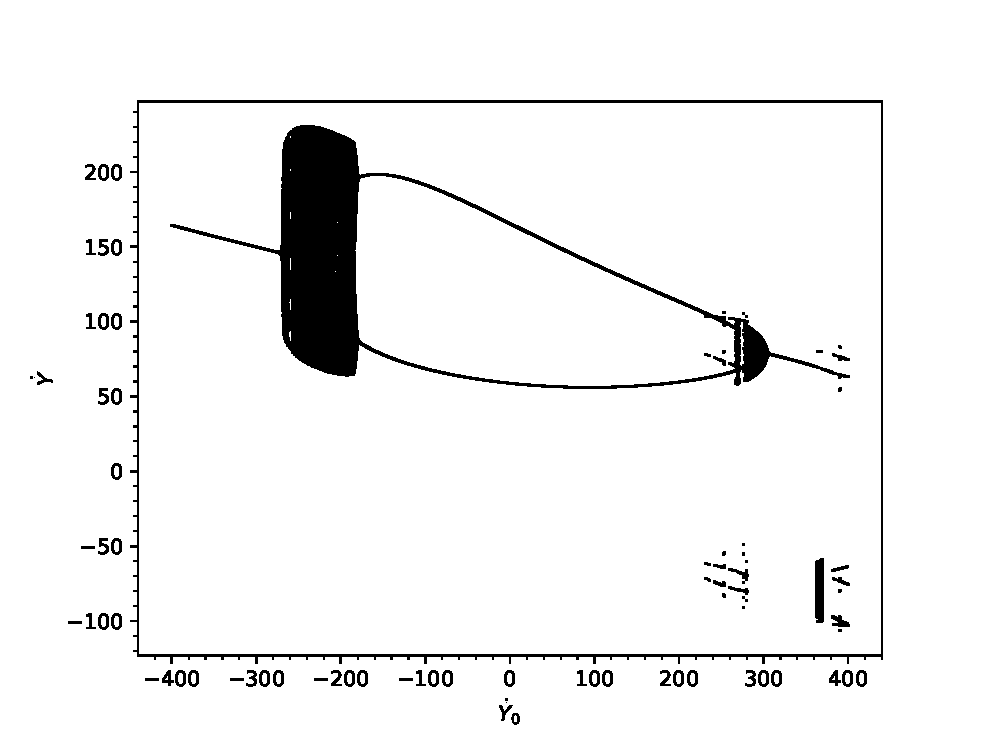
\includegraphics[height=0.4\textheight]{./metzlerian_growth/y0bifurcation}
    \caption{Bifurcation diagram varying $\dot Y_0$ between -400 and 400. All other parameters and initial conditions kept as described in Figure \ref{growth_timeseries1}}
    \label{metzlerian_growth-y0bifurcation}
\end{figure}

This diagram shows several clearly defined regions of stable, ordered behavior. There is a bifurcation when $Y_0\approx -267.986$ that causes the dynamics of the mapping to shift away from fixed, stable growth. There is also a region where stable 2-cycles exist between -180.378 and 231.903 before the emergence of higher order cycles. 

\begin{figure}
    \centering
    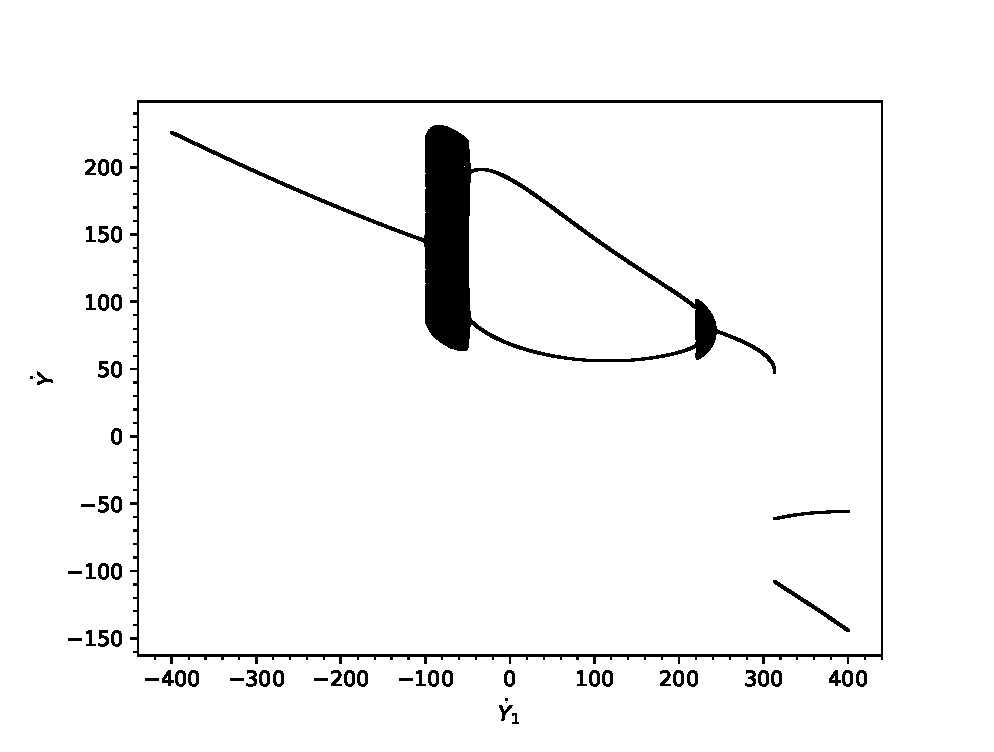
\includegraphics[height=0.4\textheight]{./metzlerian_growth/y1bifurcation}
    \caption{Bifurcation diagram varying $\dot Y_1$ between -400 and 400. All other parameters and initial conditions kept as described in Figure \ref{growth_timeseries1}}
    \label{metzlerian_growth-y1bifurcation}
\end{figure}

Figure \ref{metzlerian_growth-y1bifurcation} is also relatively simple to analyze, featuring a fixed growth rate until the bifurcation point where $Y_1\approx -99.010$. A region of stable 2-cycles also exist when $Y_1\in(-48.205,220.542)$. Fixed growth recommences when $Y_1\approx 243.104$ before shifting back into a 2-cycle region when $Y_1\approx 313.351$. 

\begin{figure}
    \centering
    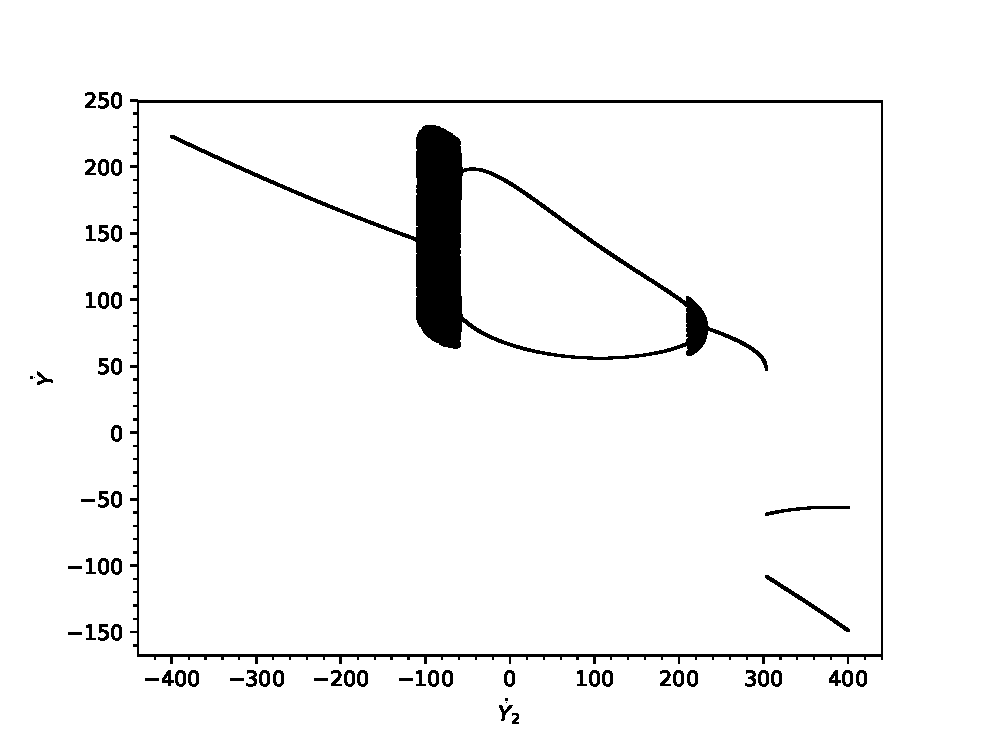
\includegraphics[height=0.4\textheight]{./metzlerian_growth/y2bifurcation}
    \caption{Bifurcation diagram varying $\dot Y_2$ between -400 and 400. All other parameters and initial conditions kept as described in Figure \ref{growth_timeseries1}}
    \label{metzlerian_growth-y2bifurcation}
\end{figure}

Figure \ref{metzlerian_growth-y2bifurcation} is qualitatively almost identical to the diagram displayed in Figure \ref{metzlerian_growth-y1bifurcation}. The model displays fixed growth until the bifurcation point when $Y_2\approx -109.011$. A region of stable 2-cycles exists when $Y_2\in(-58.206, 210.541)$. Fixed growth recommences after the bifurcation point when $Y_2\approx 233.103$ before shifting back into stable 2-cycles when $Y_2\approx 303.350$. 

\begin{figure}
    \centering
    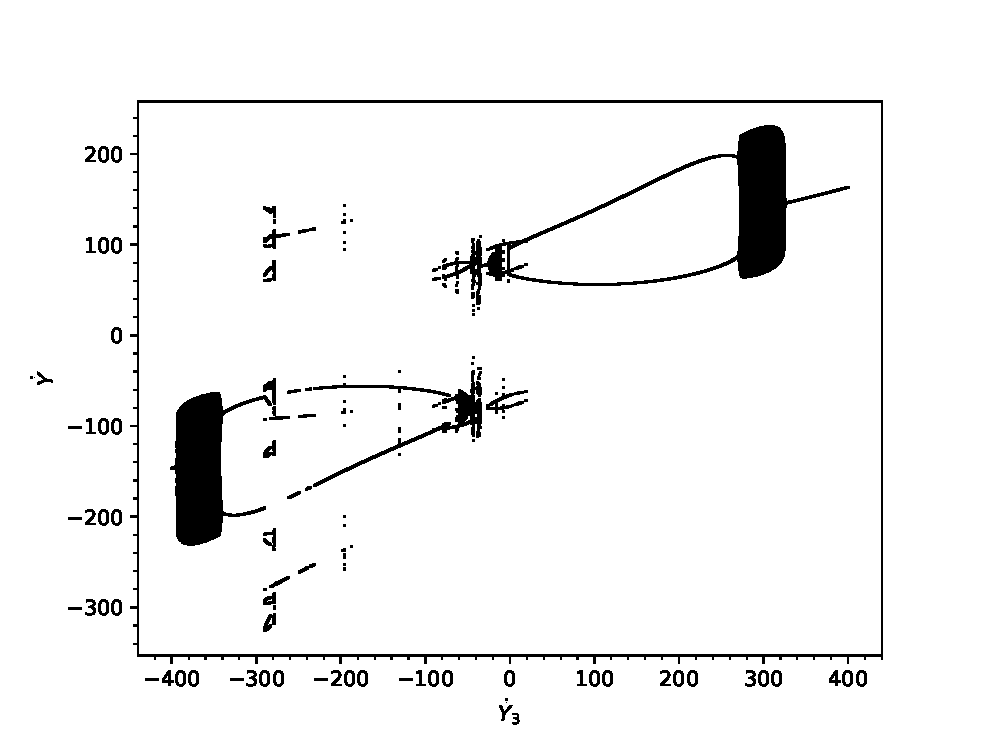
\includegraphics[height=0.4\textheight]{./metzlerian_growth/y3bifurcation}
    \caption{Bifurcation diagram varying $\dot Y_3$ between -400 and 400. All other parameters and initial conditions kept as described in Figure \ref{growth_timeseries1}}
    \label{metzlerian_growth-y3bifurcation}
\end{figure}

Figure \ref{metzlerian_growth-y3bifurcation} possess many regions of clearly visible, ordered cyclic behavior, of note however is presence of stable 2-cycles when $Y_3\in (19.162, 270.867$.

\begin{figure}
    \centering
    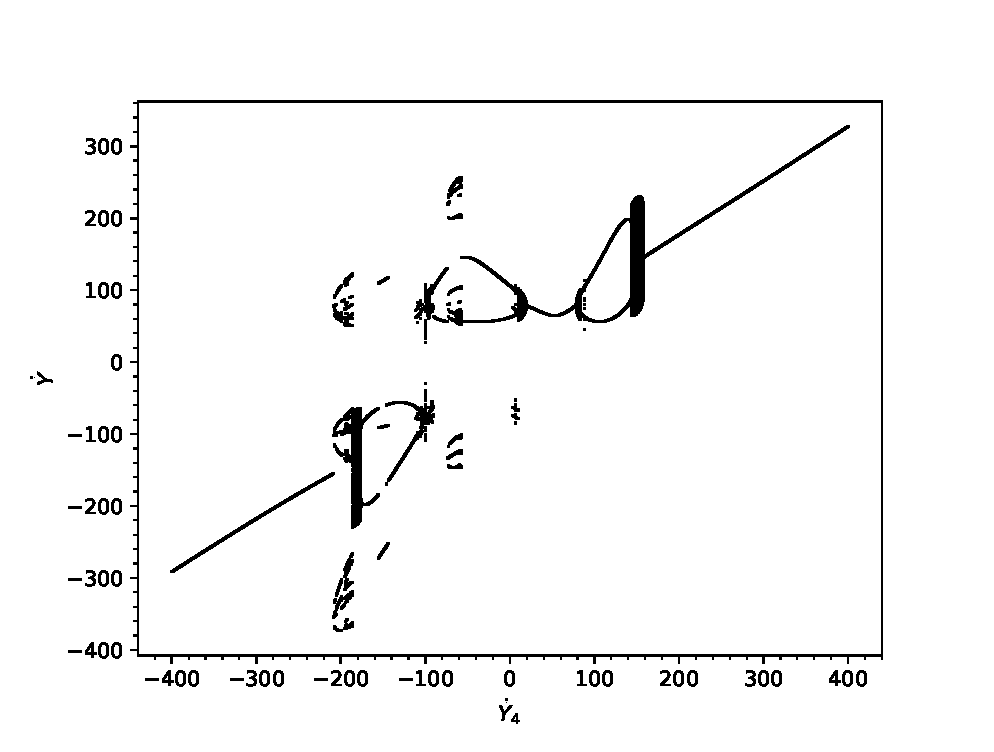
\includegraphics[height=0.4\textheight]{./metzlerian_growth/y4bifurcation}
    \caption{Bifurcation diagram varying $\dot Y_4$ between -400 and 400. All other parameters and initial conditions kept as described in Figure \ref{growth_timeseries1}}
    \label{metzlerian_growth-y4bifurcation}
\end{figure}

\section{Chaotic Behavior in Growth}
Bifurcation analysis of this type allows us to determine the presence and location of bifurcation points separating arbitrary period cycles. However, this is insufficient to determining if varying the parameters of the model result in chaotic behavior and where exactly this transition occurs. The existence of chaos lends credence to the assumption of bounded rationality assigned to firms. If the model always features stable cycles, then it would only be logical that firms would eventually be able to adapt their predictive mechanism to predict this ordered behavior. The effect this shift in expectation rule would have on future dynamics is beyond the scope of this paper; however, the presence of chaos means the model is sufficiently sensitive to initial conditions that firms would not be able to accurately determine the future state of the market as under a chaotic system, knowing the approximate current state of the economy does not inform firms of the approximate future state of the economy. 

The method described in the introduction to solve for the lyapunov exponent is applicable to 1-dimensional systems. Although are system is formally a 1-dimensional, 6th order difference equation, existing methods of analysis are much more accomodating to single-order mappings. We thus begin by rewriting the model as a 1st-order difference equation with 6 variables. This can be done by creating and defining the variables $\dot Y_{t-1}=\dot A_t$, $\dot A_{t-1}=\dot B_{t}$, $\dot B_{t-1}=\dot C_{t}$, $\dot C_{t-1}=\dot D_{t}$, and $\dot D_{t-1}=\dot G_{t}$. This allows us to define an equivalent model:
\begin{align*}
    \dot Y_t = f(\dot Y_{t-1}, \dot A_{t-1}, \dot B_{t-1}, \dot C_{t-1}, \dot D_{t-1}, \dot G_{t-1})\\
    \dot A_t = g(\dot Y_{t-1}, \dot A_{t-1}, \dot B_{t-1}, \dot C_{t-1}, \dot D_{t-1}, \dot G_{t-1})\\
    \dot B_t = h(\dot Y_{t-1}, \dot A_{t-1}, \dot B_{t-1}, \dot C_{t-1}, \dot D_{t-1}, \dot G_{t-1})\\
    \dot C_t = j(\dot Y_{t-1}, \dot A_{t-1}, \dot B_{t-1}, \dot C_{t-1}, \dot D_{t-1}, \dot G_{t-1})\\
    \dot D_t = l(\dot Y_{t-1}, \dot A_{t-1}, \dot B_{t-1}, \dot C_{t-1}, \dot D_{t-1}, \dot G_{t-1})\\
    \dot G_t = m(\dot Y_{t-1}, \dot A_{t-1}, \dot B_{t-1}, \dot C_{t-1}, \dot D_{t-1}, \dot G_{t-1})
\end{align*}
The Jacobian matrix of this system of equations is:
\begin{equation*}
J = \begin{bmatrix}
    \frac{\partial f}{\partial \dot Y_{t-1}} & \frac{\partial f}{\partial \dot A_{t-1}} & \frac{\partial f}{\partial \dot B_{t-1}} & \frac{\partial f}{\partial \dot C_{t-1}} & \frac{\partial f}{\partial \dot D_{t-1}} & \frac{\ f}{\partial \dot G_{t-1}}\\
    \frac{\partial g}{\partial \dot Y_{t-1}} & \frac{\partial g}{\partial \dot A_{t-1}} & \frac{\partial g}{\partial \dot B_{t-1}} & \frac{\partial g}{\partial \dot C_{t-1}} & \frac{\partial g}{\partial \dot D_{t-1}} & \frac{\ f}{\partial \dot G_{t-1}}\\
    \frac{\partial h}{\partial \dot Y_{t-1}} & \frac{\partial h}{\partial \dot A_{t-1}} & \frac{\partial h}{\partial \dot B_{t-1}} & \frac{\partial h}{\partial \dot C_{t-1}} & \frac{\partial h}{\partial \dot D_{t-1}} & \frac{\ f}{\partial \dot G_{t-1}}\\
    \frac{\partial j}{\partial \dot Y_{t-1}} & \frac{\partial j}{\partial \dot A_{t-1}} & \frac{\partial j}{\partial \dot B_{t-1}} & \frac{\partial j}{\partial \dot C_{t-1}} & \frac{\partial j}{\partial \dot D_{t-1}} & \frac{\ f}{\partial \dot G_{t-1}}\\
    \frac{\partial l}{\partial \dot Y_{t-1}} & \frac{\partial l}{\partial \dot A_{t-1}} & \frac{\partial l}{\partial \dot B_{t-1}} & \frac{\partial l}{\partial \dot C_{t-1}} & \frac{\partial l}{\partial \dot D_{t-1}} & \frac{\ f}{\partial \dot G_{t-1}}\\
    \frac{\partial m}{\partial \dot Y_{t-1}} & \frac{\partial m}{\partial \dot A_{t-1}} & \frac{\partial m}{\partial \dot B_{t-1}} & \frac{\partial m}{\partial \dot C_{t-1}} & \frac{\partial m}{\partial \dot D_{t-1}} & \frac{\ f}{\partial \dot G_{t-1}}
\end{bmatrix}
\end{equation*}
\begin{equation}
J=
\begin{bmatrix}\small
    \frac{\partial f}{\partial Y_{t-1}} & \frac{\partial f}{\partial A_{t-1}} & s+\frac{k+1}{3}s & 0 & \frac{(k+1)(s-1)}{3} & -\frac{(k+1)s}{3}\\
    1 & 0 & 0 & 0 & 0 & 0\\
    0 & 1 & 0 & 0 & 0 & 0\\
    0 & 0 & 1 & 0 & 0 & 0\\
    0 & 0 & 0 & 1 & 0 & 0\\
    0 & 0 & 0 & 0 & 1 & 0
\end{bmatrix}
\end{equation}
where 
\begin{align*}
    \frac{\partial f}{\partial Y_{t-1}}&= \frac{1}{v\left(q+\frac{Y_{t-1}^4}{v^4}\right)}-\frac{4Y_{t-1}^4}{v^5\left(q+\frac{Y_{t-1}^4}{v^4}\right)}\\
    \frac{\partial f}{\partial A_{t-1}}&=1+\frac{1}{3}(k+1)(1-s)-s+\frac{4A_{t-1}^4}{v^5\left(q+\frac{A_{t-1}^4}{v^4}\right)^2}-\frac{1}{v\left(q+\frac{A_{t-1}^4}{v^4}\right)}
\end{align*}

Figure \ref{derivative1} and \ref{derivative2} displays the possible values for the variable partial derivatives of the model over a reasonable range of growth rates. All other partial derivatives present in the Jacobian are clearly constant given a set of parameters.

\begin{figure}[h]
    \centering
    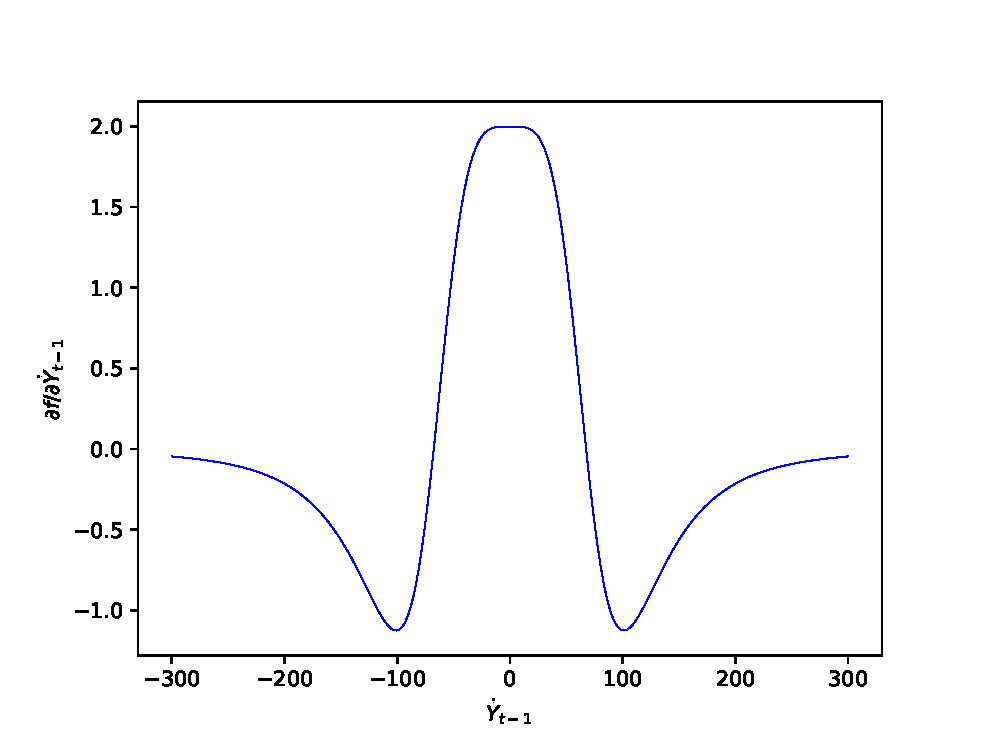
\includegraphics[height=0.4\textheight]{./metzlerian_growth/derivative1.eps}
    \caption{Plot of $\frac{\partial f}{\partial \dot Y_{t-1}}$ with respect to $\dot Y_{t-1}$.}
    \label{derivative1}
\end{figure}

\begin{figure}
    \centering
    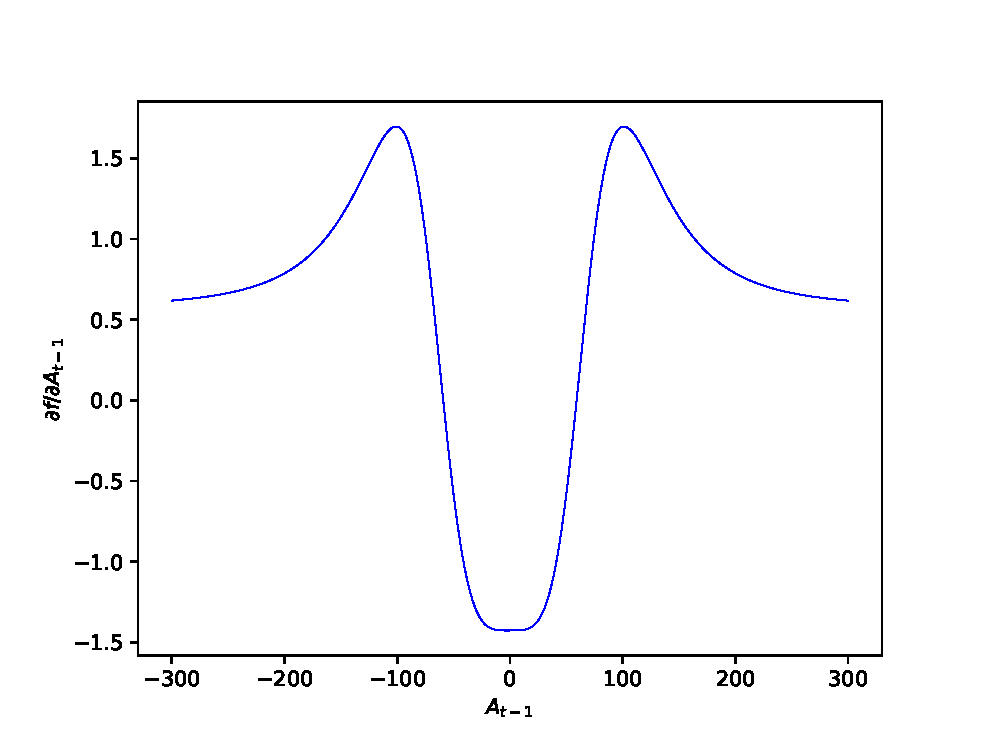
\includegraphics[height=0.4\textheight]{./metzlerian_growth/derivative2.eps}
    \caption{Plot of $\frac{\partial f}{\partial \dot A_{t-1}}$ with respect to $\dot A_{t-1}=\dot Y_{t-2}$.}
    \label{derivative2}
\end{figure}

If we think of the our mapping as a transformation of an $n$-dimensional space and the lyapunov exponent as a measure of the compression and expansion of this space, it is clear that we must track the direction of this action as the transformation iterates through time. This is accomplished by evaluating the evolution of an $n$-length vector $v$, normalized to a length of 1 for simplicity as the direction of this vector is all we are concerned with. This occurs with the 1-dimensional case as well, by incorporating a 1-dimensional vector of length 1. This is however, equivalent to the scalar 1 so it need not be explicitly included in calculation for reasons that will be elaborated here. The Jacobian $J$ operates as the higher-dimension analogue to the derivative so by taking the product of the Jacobian and the direction vector, we are able to project our derivatives onto the direction vector. From here, we can solve for the lyapunov exponent much like in our 1-dimensional case:
\begin{equation}
    \lambda = \lim_{j\to\infty}\frac{1}{j}\sum^{t=j}_{j=1}\ln\lvert J_t\cdot v_t\rvert
\end{equation}
With a 1-dimensional mapping, $v_t=v=1$ and $J_t=f^\prime(x_t)$. It is clear how the Jacobian evaluates over time, changing over the course of the time-series. The direction vector must also be updated, this is accomplished by normalizing the length of the projection:
\begin{equation}
    v_{t+1}=\frac{J_t\cdot v_t}{\lvert J_t\cdot v_t\rvert}
\end{equation}
A consequence of this is that the lyapunov exponent is now both dependent on the initial condition and the choice of initial direction vector. As stated in the introduction, the inital condition provided it not reside in an unstable periodic cycle; moreover, the choice of intial vector is of little consequence as it quickly updates to the correct elongation direction regardless of intiial choice. As stated for the 1-dimensional case, it is typically impractical to solve for the lyapunov exponent analytically; however, we can approximate it by iterating the model for some large $t$ and treating this value as the limit.

An important note is that although 1-dimensional models only have 1 lyapunov exponent, $n$ dimensional models actually have $n$ lyapunov exponents.The method described above only calculates the largest exponent; however, it is typically only necessary to determine this maximal value as the positivity of this exponent is used as the determiner of chaos in the system. A consequence of the bounded behavior of our model is that the negative lyapunov exponents must "dominate" in order to result in overall compression of the model; otherwise the mapping would result in an explosive model. 

\begin{figure}
    \centering
    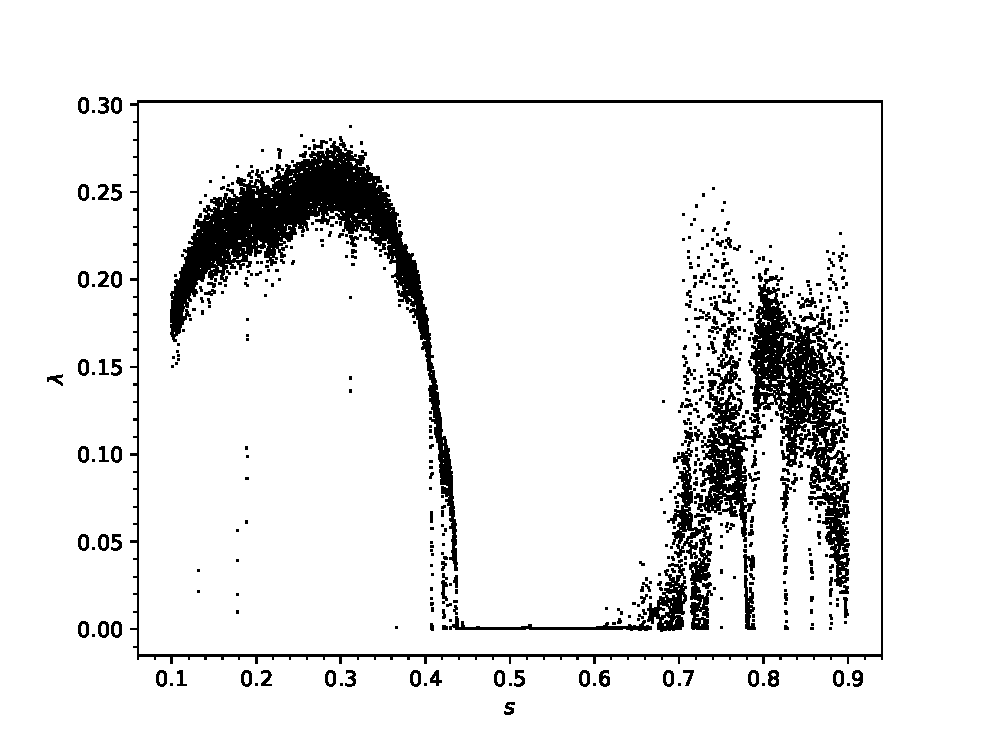
\includegraphics[height=0.4\textheight]{./metzlerian_growth/slyplot.eps}
    \caption{Lyapunov plot varying $s$ between 0 and 1. Other parameters and initial conditions are held constant held constant as described in Figure \ref{growth_timeseries1}.}
    \label{slyapunov}
\end{figure}
\begin{figure}
    \centering
    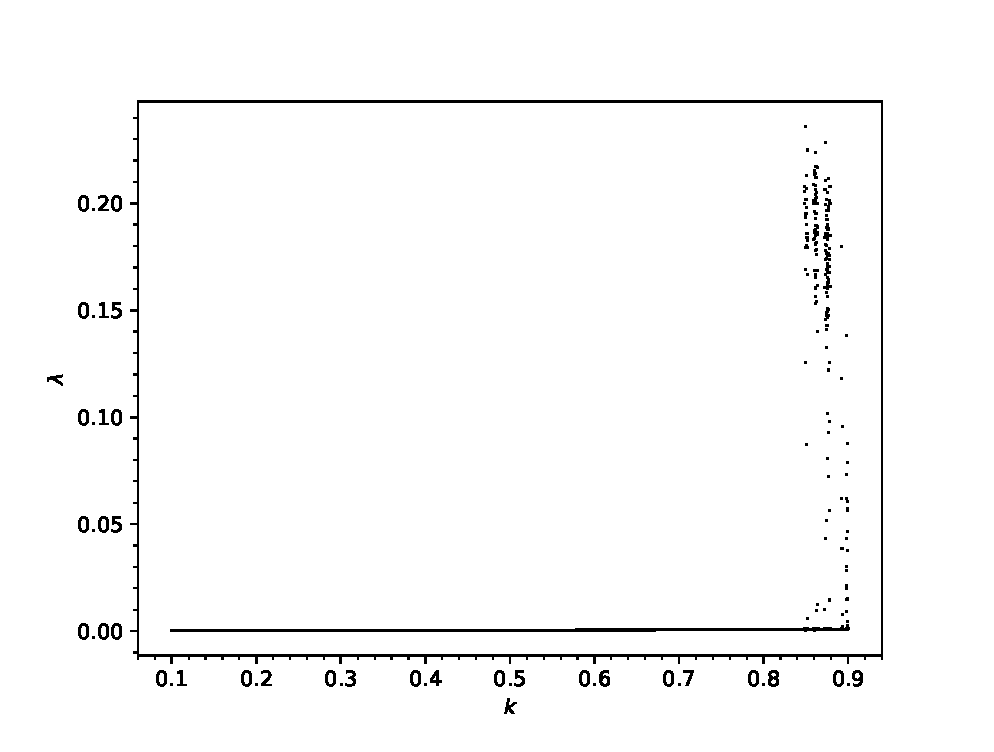
\includegraphics[height=0.4\textheight]{./metzlerian_growth/klyplot.eps}
    \caption{Lyapunov plot varying $k$ between 0 and 1. Other parameters and initial conditions are held constant held constant as described in Figure \ref{growth_timeseries1}}
    \label{klyapunov}
\end{figure}
\begin{figure}
    \centering
    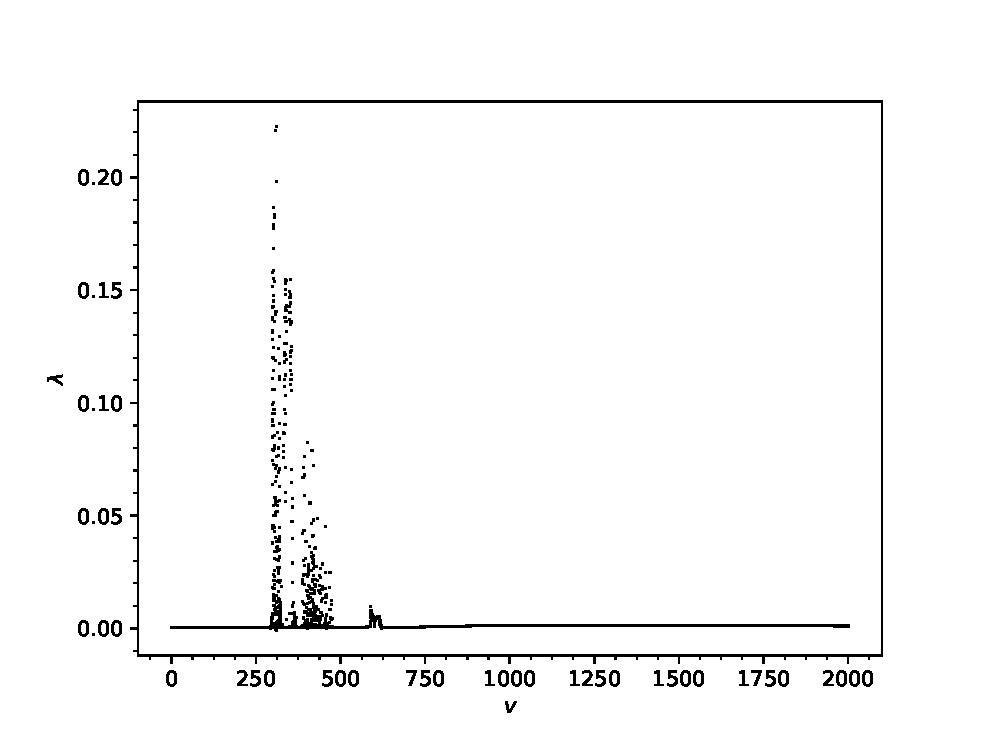
\includegraphics[height=0.4\textheight]{./metzlerian_growth/vlyplot.eps}
    \caption{Lyapunov plot varying $v$ between 1 and 2000. Other parameters and initial conditions are held constant held constant as described in Figure \ref{growth_timeseries1}}
    \label{klyapunov}
\end{figure}
\begin{figure}
    \centering
    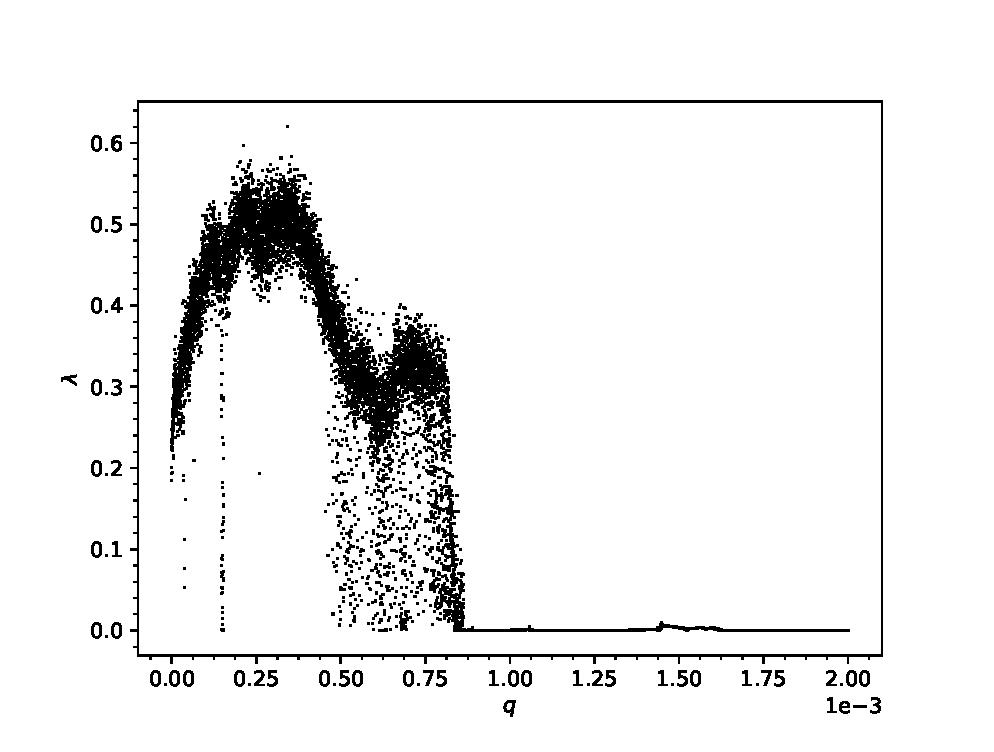
\includegraphics[height=0.4\textheight]{./metzlerian_growth/qlyplot.eps}
    \caption{Lyapunov plot varying $q$ between 0 and 0.002. Other parameters and initial conditions are held constant held constant as described in Figure \ref{growth_timeseries1}}
    \label{klyapunov}
\end{figure}

Note again that we are calculating only the maximal Lyapunov exponent, thus if the displayed lyapunov exponent is 0, the other exponents may be 0 or even negative meaning that there can be compression of the space occuring even when $\lambda=0$. 











\chapter{Conclusion}
One of the core debates of economic theory is that of the rationality of agents. Keynesian economics was the dominant school of thought until the 1970s which saw the rise of New Classical economics\autocite{Hartley2013}. Lucas and Sargent were two key spearheads of this movement with their influential paper titled "After Keynesian Macroeconomics", key to their complaints were the lack of microeconomic foundations in Keynesian models\autocite{Lucas1979}. Real business cycle theory, a major branch of New Classical economics believed that business cycles were a rational response to exogenous shocks to the economy and were perfectly efficient. However, this also meant that business cycles would not arise endogenously as firms and consumers would learn over time the behavior of the economy as they, as a whole, acted rationally. Though Keynesianism has since gained in popularity after the 2007 financial crisis, these lessons of New Classical Economics continue to influence the microfoundations of macroeconomic New Keynesian models.

Wegener, et al. directly based their inventory cycle model on that developed by Metzler. However, both of these models required that firms be boundedly rational which, to a New Classical economist, would be an unrealistic assumption not rooted in microeconomic foundations. However, it is appropriate to limit the ability for firms to predict the future if the reason for it can be appropriately explained. Behavioral economics and experimental data has frequently shown a gap between perfectly rational, utilitarian behavior and what is actually practiced by humans\autocite{Smith2006}; however, we would expect firms to behave more rationally than individuals. Some models make use of stochastic shocks in order to drive dynamic behavior; these tend to follow a New Classical real business cycle framework as these stochastic processes are the primary drivers of economic cycles. Another possible process is that of chaotic behavior. Under these conditions, it is possible for the economy to reside in a completely deterministic state while still making it impossible for firms to accurately predict future states in the economy . Having the unpredictability of the economy be primarily driven by chaotic processes rather than stochastic ones is of great use from a policy perspective due to the nature of having parameters to influence rather than random behavior, this is discussed in greater detail by Faggini and Parziale\autocite{Faggini2012}. 

The growth model described in Chapter \ref{ch:metzlerian-expanded} has a basis in Metzler's inventory cycle but also incorporates a multiplier-accelerator mechanism for endogenous investment and consumption and the results of numerical simulations of the model display the possibility of chaos, in addition to other phenomena such as the existence of multiple attractors. Of particular note is the bifurcation diagram and Lyapunov exponent plot of the parameter $s$. The marginal propensity to save, under the initial conditions and other parameter choice tested, do not display any stable fixed points. In fact, over the possible range of $s$, most possible trajectories are chaotic; one such trajectory is displayed in Figure \ref{growth_chaotic-timeseries}.
\begin{figure}
    \centering
    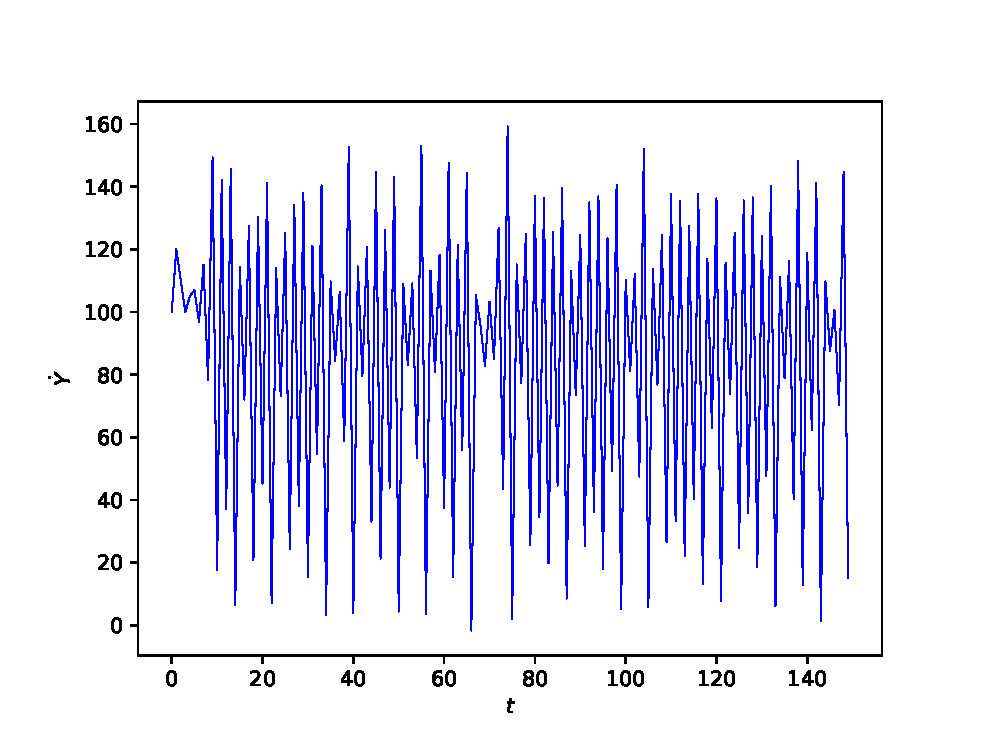
\includegraphics[height=0.4\textheight]{./metzlerian_growth/chaotic_timeseries.eps}
    \caption{Timeseries plot of income growth rate over 150 iterations. $s=0.4,\ k=0.3,\ v=500,\ q=0.001$. Initial values of $\dot Y$ are: 100, 120, 110, 100, 105, 107}
    \label{growth_chaotic-timeseries}
\end{figure}
Figure \ref{metzlerian_growth-kLyapunov} also displays chaotic behavior; however, this only occurs when $k$ is very large and is unlikely to occur in a real scenario. Both $s$ and $k$ are the two parameter choices that describe the behavior of the agents of the economy in non-monetary terms. Based on the results of Figure \ref{metzlerian_growth-kLyapunov} and \ref{metzlerian_growth-kbifurcation}, variation of this parameter has minor effects on the growth rate of the economy compared to variation of $s$. This implies that the choice of inventory proportion, outside of the extreme cases, has a minor impact on the long-run dynamics of the model. This is not to say that the inventory cycle is itself a minor factor of the economy; removal of the inventory cycle changes this model to an unsimplified version of the model presented in Chapter \ref{ch:multiplier-accelerator}. This model features a functionally identical mechanism for consumption with a Robertson lag and although the form of the function for endogenous investment differs between the two models, they are qualitatively similar for the reasons mentioned in Chapter \ref{ch:metzlerian-expanded}.

\begin{figure}
    \centering
    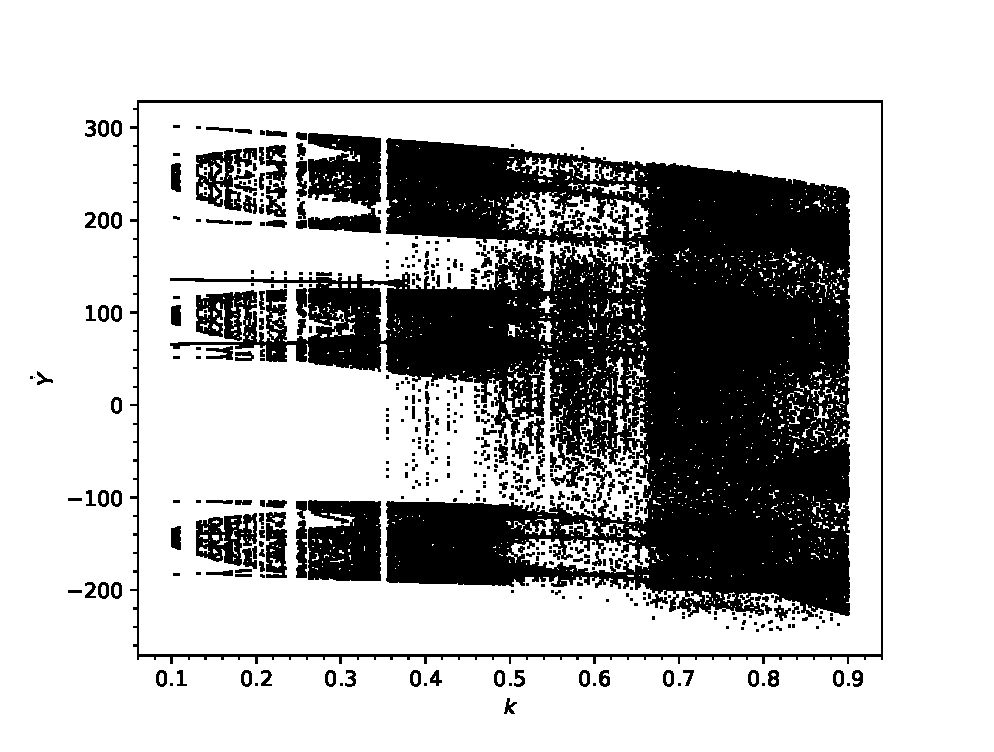
\includegraphics[height=0.4\textheight]{./metzlerian_growth/kbifurcation2.eps}
    \caption{Bifurcation diagram varying $k$ between 0.1 and 0.9. Initial conditions and other parameters are held constant as described in Figure 4.1 except $s=0.7$}
    \label{metzlerian_growth-kbifurcation2}
\end{figure}
\begin{figure}
    \centering
    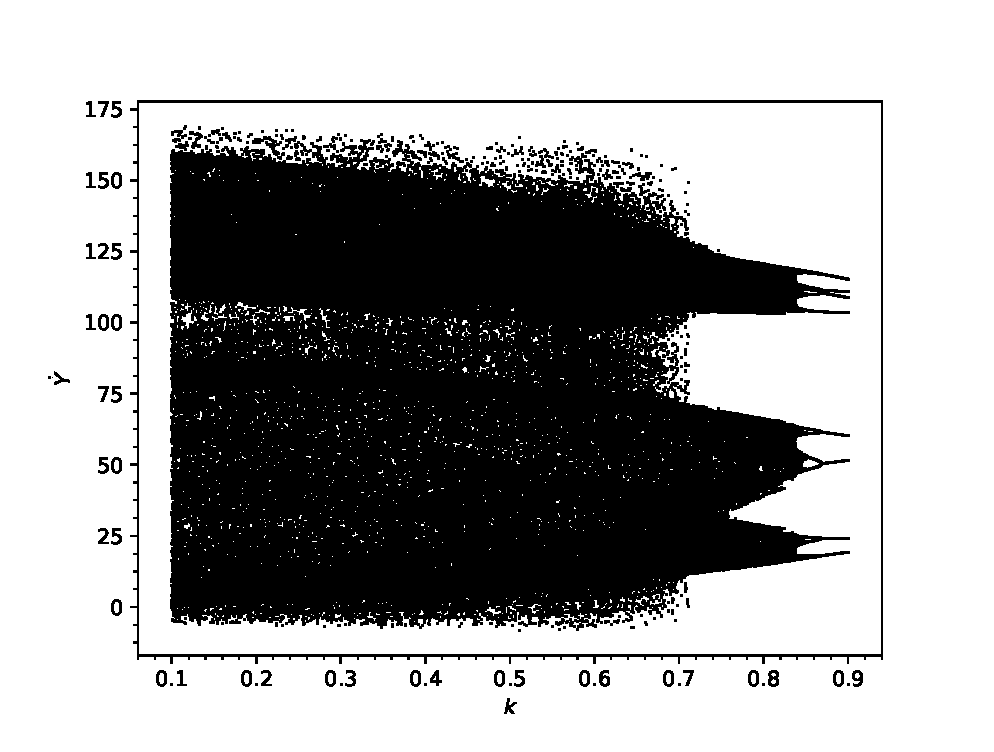
\includegraphics[height=0.4\textheight]{./metzlerian_growth/kbifurcation3.eps}
    \caption{Bifurcation diagram varying $k$ between 0.1 and 0.9. Initial conditions and other parameters are held constant as described in Figure 4.1 except $s=0.3$}
    \label{metzlerian_growth-kbifurcation3}
\end{figure}
Figure \ref{metzlerian_growth-kbifurcation2} and \ref{metzlerian_growth-kbifurcation3} displays behavior that is qualitatively distinct from that in Figure \ref{metzlerian_growth-kbifurcation} despite both plots showing the long-run behavior of the model with the same variation in $k$. However, by increasing or decreasing $s$ until it is in the chaotic regime presented in Figure \ref{metzlerian_growth-sLyapunov}, we see that varying $k$ can have a significant effect on the long-run dynamics of growth at even more reasonable values of $k$.

$q$ determines the maximum and minimum of the investment function and $v$ is the primary determinant of of the FWHM of the function. Given the initial conditions, we see chaotic behavior when large quantities of investment are allowed by the investment curve, i.e. $q$ is small. The initial growth values vary between 100 and 120 so it appears that allowing investment to exceed growth in quantity results in instability;  however, there do still remain windows of order in the primary chaotic region of $q$. Interestingly, the system appears to be relatively ordered for most values of $v$; however, there is a small region where $250<v<750$ that displays chaotic behavior in Figure \ref{metzlerian_growth-vLyapunov}. Figure \ref{metzlerian_growth-chaotic_timeseries2} displays one such trajectory, of note is how the model cycles between both positive and negative growth regimes but also between high amplitude variation and low amplitude variation. It appears that under this parametrization, high absolute values of income change reduce investment; however, instead of ending in stability, this lower income variance state drives higher levels of investment shifting the model back to a high income variance regime.
\begin{figure}
    \centering
    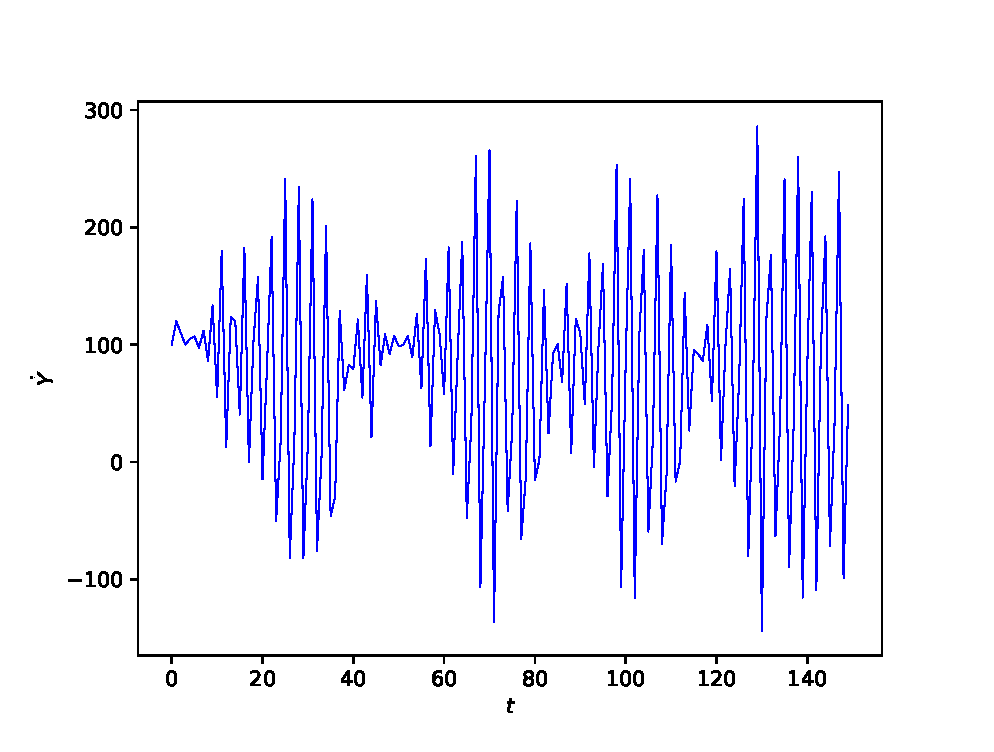
\includegraphics[height=0.4\textheight]{./metzlerian_growth/chaotic_timeseries2.eps}
    \caption{Timeseries plot of income growth rate over 150 iterations. $s=0.6,\ k=0.3,\ v=416,\ q=0.001$}
    \label{metzlerian_growth-chaotic_timeseries2}
\end{figure}

$v$ and $q$ are likely to change depending on the state of the economy, the government's fiscal policy, and the technology available. The investment curve bends back and has a "width" due to the presumption of changes in public investment and taxes in response to the state of the economy and the presence of other limiting factors in income growth. If the government decides to loosen their concern to output variation, the width of the investment curve would increase. The height of the function can change over time as the required level of investment needed to sustain an output level changes can change with improvements in technology or human capital. 

Generally speaking, larger values of early initial growth compared to the later values of initial growth results in a lower overall long-run growth. This can be seen in Figure \ref{metzlerian_growth-y0bifurcation}, \ref{metzlerian_growth-y1bifurcation}, and \ref{metzlerian_growth-y2bifurcation}. The relationship is reversed if growth is larger for more recent time periods as can be seen in Figure \ref{metzlerian_growth-y3bifurcation}, \ref{metzlerian_growth-y4bifurcation}, and \ref{metzlerian_growth-y5bifurcation}. Ignoring the chaotic behavior, this model implies that relatively sharp drops in growth rate result in lower growth horizons whereas large spikes in growth rate result in high growth horizons. The non-linear nature of the model and presence of multiple attractors complicates this idea although the trend is still present. This economy is susceptible to external forces; an exogenous but temporary increase in the growth rate will result in a long-run increase in growth rate. The economy is thus able to use aid in order to accelerate its own growth. Likewise, if an external shock reduces output relative to its usual behavior, this can result in a decreased growth rate in the long-run. 

The goal of this model was to incorporate both a Robertson and Lundberg lag and endogenize investment change. This was done in order to provide a mechanism to explain why firms on aggregate are unable to accurately predict future consumption. Many models use stochastic processes in order to rationalize this; however, this model shows the presence of chaotic behavior. Under a chaotic regime, firms would only be able to predict future behavior by knowing the exact state of the economy in the past; however, this is practically impossible as even small differences between the actual initial conditions and estimated initial conditions will result in very different future results by the definition of chaos. 

Much work remains to be done on this model in order to better describe the quantity and structure of the multiple attractors and an explanation of the model's response to changing parameters. As more work is done on the mathematics of higher-order non-linear iterated maps, it may become possible to analytically solve for the behavior of the model although this remains unlikely for the near future. More work also needs to be done to differentiate between quasi-periodic behavior and chaotic behavior in the model, although both are inherently unpredictable, quasi-periodic behavior provides a more consistent structure to long-run behavior while still preventing firms from accurately determining future outcomes.

This model could also be expanded upon in a variety of ways. This economy is closed; however, most modern economies are open to foreign trade to varying degrees. This provides another income channel as well as providing another outlet for investment that does not improve the domestic economy. A more complex investment mechanism could also be incorporated, by explicitly separating public and private investments and removing the x-axis symmetry seen in the current curve. There are many possible ways for firms to predict future consumption, a simple average was used here although a conditional expectation that would allow firms to better use past information and learn from their previous experiences would help alleviate concerns regarding rational behavior by the firms. This however can lead to mathematical complications if firms have infinite possible memory. These additions could improve the realism of the model while still using chaos as the primary driver of chaotic behavior. 




\chapter{References}
\thispagestyle{empty}
\printbibliography[heading=none]
\begin{appendices}
\chapter{Solving for Change in Income}
We can define the growth rate $\dot Y_t$ as the difference in income between contiguous time periods:
\begin{equation}
    \dot Y_t=Y_{t+1}-Y_t
\end{equation}
Let this dot notation refer to the analogous growth rate of other state variables. This equation can be expanded using Equation \ref{eq:Income}.
\begin{equation*}
    \dot Y_t=(U_{t+1}-U_t)+(I_{t+1}-I_t)+(S_{t+1}-S_t)=\dot U_t+\dot I_t+\dot S_t
\end{equation*}

The change in investment can be trivially solved for as investment is already a function of the change in income.
\begin{equation*}
    I_t=\frac{\frac{\dot Y_{t-2}}{v}}{\left(\frac{\dot Y_{t-2}}{v}\right)^4+q}
\end{equation*}
Thus the change in investment is:
\begin{equation}
    \dot I_t=\frac{\frac{\dot Y_{t-1}}{v}}{\left(\frac{\dot Y_{t-1}}{v}\right)^4+q}-\frac{\frac{\dot Y_{t-2}}{v}}{\left(\frac{\dot Y_{t-2}}{v}\right)^4+q}
\end{equation}

As predicted consumption is a function of the change in actual consumption, we must derive a function for the change in consumption in terms of the growth rate.
\begin{equation*}
    C_{t+1}-C_t=[(1-s)Y_{t}+sY_{t-1}]-[(1-s)Y_{t-1}+sY_{t-2}]
\end{equation*}
This can be simplified to:
\begin{equation}
    \dot C_t=(1-s)(Y_{t}-Y_{t-1})+s(Y_{t-1}-Y_{t-2})=(1-s)\dot Y_{t-1} + s\dot Y_{t-2}
\end{equation}

The change in expected consumption can be given by:
\begin{align*}
    U_{t+1}-U_{t}&=\frac{C_{t}+C_{t-1}+C_{t-2}}{3}-\frac{C_{t-1}+C_{t-2}+C_{t-3}}{3}\\
    \dot U_t&=\frac{\dot C_{t-1}+\dot C_{t-2}+\dot C_{t-3}}{3}
\end{align*}
This can be clearly resolved into a function of income growth rates:
\begin{equation*}
    \dot U_t=\frac{[(1-s)\dot Y_{t-2} + s\dot Y_{t-3}]+[(1-s)\dot Y_{t-3} + s\dot Y_{t-4}]+[(1-s)\dot Y_{t-4} + s\dot Y_{t-5}]}{3}
\end{equation*}
\begin{equation}
    \dot U_t=\frac{(1-s)(\dot Y_{t-2}+\dot Y_{t-3}+\dot Y_{t-4})+s(\dot Y_{t-3}+\dot Y_{t-4}+\dot Y_{t-5})}{3}
\end{equation}

The final step is to solve for inventory production in terms of growth rates. We can substitute our $S_t$ into our function for $Q_t$:
\begin{align*}
    Q_t&=Q_{t-1}+(kU_t-Q_{t-1}+(U_t-C_t)\\
    Q_t&=kU_t+U_t-C_t
\end{align*}
This gives an equation for the rate of change:
\begin{align*}
    Q_{t+1}-Q_{t}&=\left[kU_{t+1}+U_{t+1}-C_{t+1}\right]-\left[kU_{t}+U_{t}-C_{t}\right]\\
    \dot Q_t&= (k+1)(U_{t+1})-(k+1)(U_t)-(C_{t+1}-C_t)\\
    \dot Q_t&=(k+1)(\dot U_t)-(\dot C_t)
\end{align*}
Thus giving a function with respect to income growth rate:
\begin{equation}
\begin{split}
    \dot Q_t& = (k+1)\frac{(1-s)(\dot Y_{t-2}+\dot Y_{t-3}+\dot Y_{t-4})+s(\dot Y_{t-3}+\dot Y_{t-4}+\dot Y_{t-5})}{3}\\
    &-(1-s)\dot Y_{t-1}-s\dot Y_{t-2}
\end{split}
\end{equation}

The difference in production of goods for inventory is given by:
\begin{align*}
    S_{t+1}-S_{t}& =(kU_{t+1}-Q_{t})-(kU_{t}-Q_{t-1})\\
    \dot S_t &= k(U_{t+1}-U_t)+Q_{t-1}-Q_t\\
    \dot S_t& = k(\dot U_t)-(\dot Q_{t-1})
\end{align*}
We can thus substitute our functions for the change in predicted consumption and change in inventory:
\begin{equation}
\begin{split}
    \dot S_t& =k\frac{(1-s)(\dot Y_{t-2}+\dot Y_{t-3}+\dot Y_{t-4})+s(\dot Y_{t-3}+\dot Y_{t-4}+\dot Y_{t-5})}{3}-\\
    &\left[(k+1)\frac{(1-s)(\dot Y_{t-3}+\dot Y_{t-4}+\dot Y_{t-5})+s(\dot Y_{t-4}+\dot Y_{t-5}+\dot Y_{t-6})}{3}\right.\\
    &\left.-(1-s)\dot Y_{t-2}-s\dot Y_{t-3}\right]
\end{split}
\end{equation}

This means the function for the growth rate of the economy can be written as a 6th order, single-variable difference equation:

\begin{equation*}
\begin{split}
    \dot Y_{t}& = \frac{\frac{\dot Y_{t-1}}{v}}{\left(\frac{\dot Y_{t-1}}{v}\right)^4+q}-\frac{\frac{\dot Y_{t-2}}{v}}{\left(\frac{\dot Y_{t-2}}{v}\right)^4+q} + \\
    & \frac{(1-s)(\dot Y_{t-2}+\dot Y_{t-3}+\dot Y_{t-4})+s(\dot Y_{t-3}+\dot Y_{t-4}+\dot Y_{t-5})}{3} + \\
    &k\frac{(1-s)(\dot Y_{t-2}+\dot Y_{t-3}+\dot Y_{t-4})+s(\dot Y_{t-3}+\dot Y_{t-4}+\dot Y_{t-5})}{3}-\\
    &\left[(k+1)\frac{(1-s)(\dot Y_{t-3}+\dot Y_{t-4}+\dot Y_{t-5})+s(\dot Y_{t-4}+\dot Y_{t-5}+\dot Y_{t-6})}{3}\right.\\
    &\left.-(1-s)\dot Y_{t-2}-s\dot Y_{t-3}\right]
\end{split}
\end{equation*}
\begin{equation}
\begin{split}
    \dot Y_{t}& = \frac{\frac{\dot Y_{t-1}}{v}}{\left(\frac{\dot Y_{t-1}}{v}\right)^4+q}-\frac{\frac{\dot Y_{t-2}}{v}}{\left(\frac{\dot Y_{t-2}}{v}\right)^4+q} + \\
    & (1+k)\frac{(1-s)(\dot Y_{t-2}+\dot Y_{t-3}+\dot Y_{t-4})+s(\dot Y_{t-3}+\dot Y_{t-4}+\dot Y_{t-5})}{3} -\\
    &\left[(k+1)\frac{(1-s)(\dot Y_{t-3}+\dot Y_{t-4}+\dot Y_{t-5})+s(\dot Y_{t-4}+\dot Y_{t-5}+\dot Y_{t-6})}{3}\right.\\
    &\left.-(1-s)\dot Y_{t-2}-s\dot Y_{t-3}\right]
\end{split}
\end{equation}

\end{appendices}
\end{document}
